\chapter{Numerical experiments}
\label{chap:experiments}
This chapter presents the numerical experiments executed in order to verify the numerical methods introduced in chapter \ref{chap:discretization} as well as evaluating the a posteriori error estimates presented in chapter \ref{chap:error}. The numerical approximations were obtained using FEniCS, an automated software for solving PDEs using the Finite Element method \cite{fenics}. The aim of the experiments is to validate the convergence of the error estimates in the derived parameter-dependent norms. Also, the numerical experiments will demonstrate the potential of the a posteriori error estimators, that is, to enable intelligent control of the error in the mathematical domain. In addition to presenting the results, we will outline the methods used to obtain said results. As we are dealing with problems with no known analytic solution, we will need methods to ensure that the numerical solution is correct. 
\\
\\
All problems have been evaluated on the unit square $\Omega = (0,1)^2$. In the case of time-dependence, the domain is defined as $\Omega = (0,1)^2 \times [0, T]$, where $T$ is the total time. The mesh resolution in the numerical experiments is defined by an integer $N$ or a scalar $h$, where  $1/N=h$. The domain $\Omega$ is divided into $N \times N$ squares which again are split into two triangles by dividing each by a diagonal. The total number of triangles, or elements, will be $2N^2$ and the total number of vertices will be $(N+1)^2$. The discretization parameter $h$ is the diameter of an element, defined as the maximum length between two vertices of an element.
\\
\\
This chapter is organized as follows, section \ref{section:verification} outlines the methods of verifying the numerical solution and section \ref{section:num_exp_poisson} outlines the numerical experiment for the Poisson model. Section \ref{section:num_exp_mpet} presents numerical experiments for the MPET model with a single network and two networks. 

\section{Methods of verification} \label{section:verification}
When working with numerical simulations, it is essential to ensure that it produces reliable and trustworthy results. This can be done by checking whether the numerical simulation reproduces analytical solutions (if they exist) or if the results match experimental observations. Errors can occur in the construction of the mathematical model and the actual solving of the mathematical model \cite{oberkampf}. \textit{Validation} is the process of eliminating errors in the construction of the model, and \textit{verification} describes the methods to ensure we are solving the mathematical model correctly. This chapter will mainly focus on the latter: the process of verification. 

\subsection{Method of manufactured solutions} 
\label{section:mms}
The \textit{method of manufactured solutions} can ensure that our numerical experiment correctly solves the mathematical problem, and has been outlined in various papers cf. \cite{roache, oberkampf}. The idea is to fit the boundary conditions and source terms in accordance with a manufactured solution. This manufactured solution is an arbitrarily chosen function but needs to fulfill a few criteria. The arbitrary function typically needs to be a smooth function to ensure accuracy as well as being easy to differentiate. It should have a sufficient number of non-trivial derivatives, and it should also be non-singular. Furthermore, if the original problem contains any necessary conditions, such as e.g. divergence-free velocities or a positive solution, the manufactured solution should also fulfill this. After choosing a solution, the solver is then expected to reproduce this solution as the discretization parameter $h$ tends to zero. Computing convergence rates can verify this. We will from now on refer to the manufactured solution as the exact solution. In addition, we will use the manufactured solution as the known function on the Dirichlet boundary in the numerical experiments. 

\subsection{Convergence rate} \label{section:convergence_rate}
To verify that our numerical solvers are correct, we may check if the \textit{convergence rate} of the error is of the expected order from the a priori estimates. If an exact solution is accessible, we may quantify the error between the numerical approximation of the discrete solution $u_h$, and the exact solution, $u_e$. We obtain an "exact solution" using the method of manufactured solutions, and we may now use this to measure the error in some chosen norm,
\begin{align*}
e = \|u_h - u_e \|
\end{align*}
Any plot of error vs. mesh size (or time step) should tend to zero as the discretization approaches zero. The solver is run with decreasing discretization parameters $h$, where we compute the error with $e$ defined as above. The convergence rate is then calculated by,
\\
\begin{align*}
r(u) = \frac{\ln(e_{i+1}) - \ln(e_i)}{\ln(h_{i+1}) - \ln(h_i)}
\end{align*}
where $i$ is the refinement step and $h$ is the element diameter of the uniform mesh.
%\\
%\\
%\begin{remark}
%While it is possible to chose any manufacture solution that satisfies the conditions described in section \ref{section:mms}, it may not converge "fast enough" in certain numerical frameworks. The rate of convergence will depend on a number of factors, such as the physical parameters, the size of spatial and temporal refinement, the discretization methods as well as the manufactured solution. 
%\end{remark}
\newpage
\section{Poisson model} \label{section:num_exp_poisson} 
We solve the Poisson problem with homogeneous Dirichlet boundary conditions with a manufactured solution,
\begin{align} \label{test_poisson}
u_e = \sin(2\pi y)
\end{align}
The next step is to adjust the source terms to the exact solutions. We insert the exact solution and compute the source term:
\begin{align*}
f = 4\pi^2\sin(2\pi y)
\end{align*}
The following problems will use the same method of fitting the source terms according to the exact solution. Note that using a manufactured solution for the Poisson model is not strictly necessary as we know it to have an exact solution.
\\
\\
We derived two a posteriori estimates for the Poisson model: \eqref{eq:poisson_a_posteriori1} and \eqref{eq:poisson_a_posteriori2}, where we had the relation, 
\begin{equation}
\|u - u_h\|_{H^1} \leq c^* \eta
\end{equation}
for some a posteriori error estimator $\eta$. The two estimators $\eta_p$ and $\eta$, were defined as,  
\begin{equation}
\eta_p = \bigl\{ \sum_{T \in \mathcal{T}} h_T^2\| R_T\|^2_T + \displaystyle\sum_{E \in \mathcal{E}} h_E\| R_E \|^2_E \bigr\}^{\frac{1}{2}}
\end{equation}
and, 
\begin{equation}
\eta = \bigl\{ h_T^2 \|f_T + \Delta u_h\|_T^2  + \sum_{E \in \mathcal{E}} h_E \|R_E\|_E^2 \bigr\}^{\frac{1}{2}}
\end{equation}
Tables \ref{tab:poisson_P1}, \ref{tab:poisson_P2} and \ref{tab:poisson_P3} display the convergence rates for the a posteriori error estimators and $\|u-u_h \|_{H^1}$ approximated with $P_1$, $P_2$ and $P_3$ elements, respectively. We observe that the a priori estimates as well as the a posteriori error estimates of the error yield the optimal convergence rate when the mesh is refined. In addition, the overall accuracy of the approximation increases with higher order elements.  %The error magnitude for $\eta$ is illustrated in figures \ref{fig:poisson_eta_P1}, \ref{fig:poisson_eta_P2} and \ref{fig:poisson_eta_P3} using $P_1$, $P_2$ and $P_3$ elements, respectively. We observe a clearer resolution as we refine. The a posteriori error estimator will predict where the error is concentrated, which is indicated by the light areas. This is where we would perform adaptive refinement. 
\\
\begin{center}
\centering
\begin{tabular}{c|c|c|c|c|c|c} 
$h^{-1}$ & $\|u-u_h \|_{H^1}$ & Rate & $\eta_p$ & Rate & $\eta$ & Rate\\\hline
4 & 2.026e+0  & -     & 1.011e+1 & -     & 1.184e+1 &   -\\
8 & 1.015e+0  & 0.997 & 6.045e+0 & 0.742 & 6.246e+0 & 0.923 \\
16 & 5.049e-1 & 1.007 & 3.171e+0 & 0.931 & 3.196e+0 & 0.967\\
32 & 2.520e-1 & 1.003 & 1.605e+0 & 0.982 & 1.608e+0 & 0.991 \\
64 & 1.259e-1 & 1.001 & 8.051e-1 & 0.996 & 8.055e-1 & 0.998 \\\hline
Opt. & & 1 & & 1 & & 1
\end{tabular}
\captionof{table}{Convergence rate of the a priori and the a posteriori error estimates for the Poisson problem discretized with $P_1$ elements} \label{tab:poisson_P1}
\end{center}
\mbox{}\\
\begin{center} 
\centering
\begin{tabular}{c|c|c|c|c|c|c}
$h^{-1}$ & $\|u-u_h \|_{H^1}$ & Rate & $\eta_p$ & Rate & $\eta$ & Rate\\\hline
4  & 3.970e-1 & -     & 4.374e+0 & - 	& 5.134e+0 &   -\\
8  & 1.014e-1 & 1.969 & 1.119e+0 & 1.967 & 1.172e+0 & 2.131 \\
16 & 2.549e-2 & 1.992 & 2.799e-1 & 1.999 & 2.833e-1 & 2.049\\
32 & 6.381e-3 & 1.998 & 6.994e-2 & 2.001 & 7.016e-2 & 2.014 \\
64 & 1.596e-3 & 1.998 & 1.748e-2 & 2.000 & 1.750e-2 & 2.004  \\\hline
Opt. & & 2 & & 2 & & 2
\end{tabular}
\captionof{table}{Convergence rate of the a priori and a posteriori error estimates for the Poisson problem discretized with $P_2$ elements} \label{tab:poisson_P2}
\end{center}
\mbox{}\\
\begin{center} 
\centering
\begin{tabular}{c|c|c|c|c|c|c}
$h^{-1}$ & $\|u-u_h \|_{H^1}$ & Rate & $\eta_p$ & Rate & $\eta$ & Rate\\\hline
4  & 5.237e-2 & -     & 6.048e-1 & -     & 2.784e+0 & - \\
8  & 6.612e-3 & 2.986 & 8.382e-2 & 2.851 & 3.625e-1 & 2.941 \\
16 & 8.284e-4 & 2.997 & 1.080e-2 & 2.956 & 4.580e-2 & 2.985 \\
32 & 1.036e-4 & 2.999 & 1.362e-3 & 2.987 & 5.741e-3 & 2.996 \\
64 & 1.295e-5 & 3.000 & 1.707e-4 & 2.996 & 7.182e-4 & 2.999 \\\hline
Opt. & & 3 & & 3 & & 3
\end{tabular}
\captionof{table}{Convergence rate of the a priori and a posteriori error estimates for the Poisson problem discretized with $P_3$ elements} \label{tab:poisson_P3}
\end{center}
%\begin{figure}[h!]
%  \centering
%  \begin{subfigure}[b]{0.24\textwidth}
%    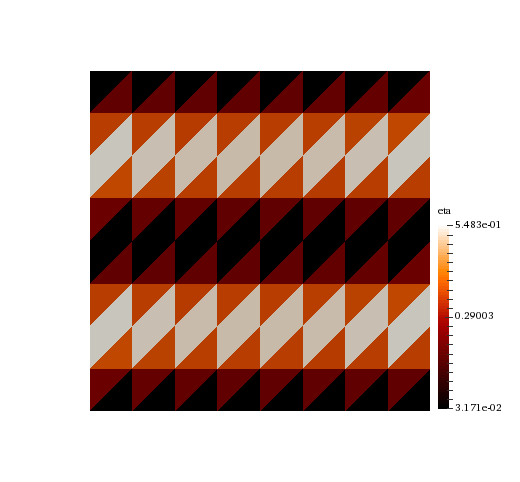
\includegraphics[width=\textwidth,height=\textheight,keepaspectratio,height=\textheight,keepaspectratio]{figures/poisson/P1/eta_8.png}
%    \caption{$N=8$}
%  \end{subfigure}
%  \begin{subfigure}[b]{0.24\textwidth}
%    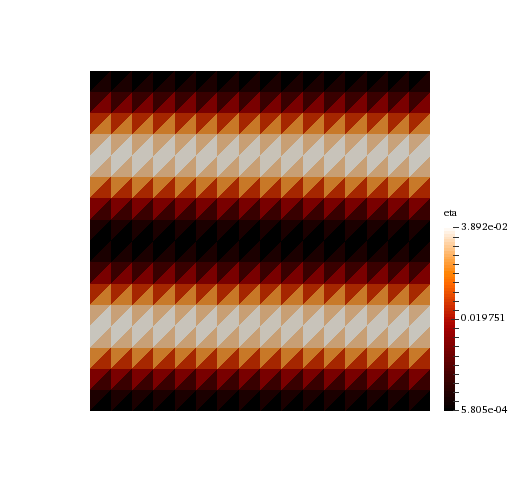
\includegraphics[width=\textwidth,height=\textheight,keepaspectratio,height=\textheight,keepaspectratio]{figures/poisson/P1/eta_16.png}
%    \caption{$N=16$}
%  \end{subfigure}
%  \begin{subfigure}[b]{0.24\textwidth}
%    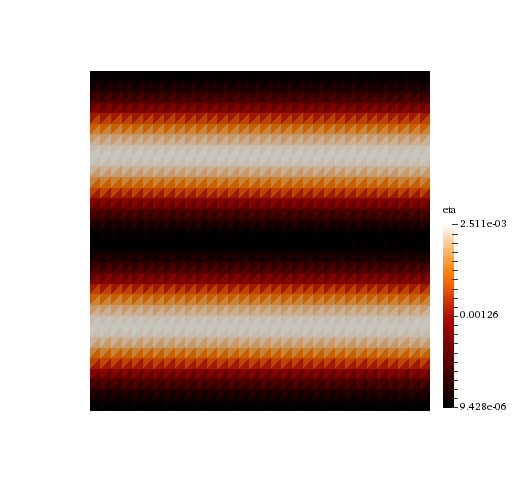
\includegraphics[width=\textwidth,height=\textheight,keepaspectratio,height=\textheight,keepaspectratio]{figures/poisson/P1/eta_32.png}
%    \caption{$N=32$}
%  \end{subfigure}
%  \begin{subfigure}[b]{0.24\textwidth}
%    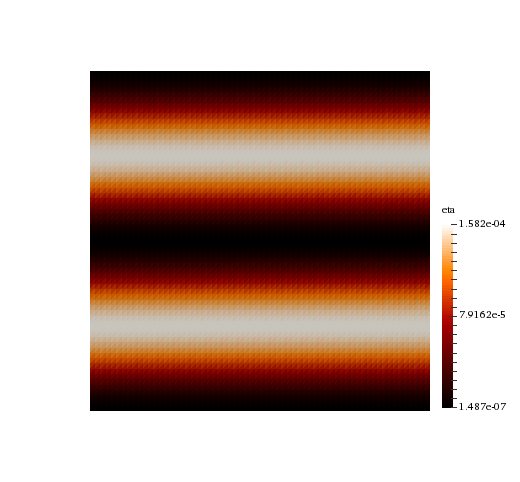
\includegraphics[width=\textwidth,height=\textheight,keepaspectratio,height=\textheight,keepaspectratio]{figures/poisson/P1/eta_64.png}
%    \caption{$N=64$}
%  \end{subfigure}
%  \caption{Error magnitude for $\eta$ for the Poisson model discretized with $P_1$ elements} \label{fig:poisson_eta_P1}
%\end{figure}
%\mbox{}\\
%\begin{figure}[h!]
%  \centering
%  \begin{subfigure}[b]{0.24\textwidth}
%    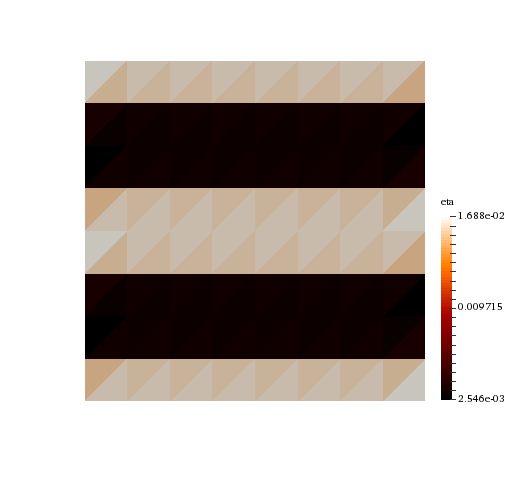
\includegraphics[width=\textwidth,height=\textheight,keepaspectratio,height=\textheight,keepaspectratio]{figures/poisson/P2/eta_8.png}
%    \caption{$N=8$}
%  \end{subfigure}
%  \begin{subfigure}[b]{0.24\textwidth}
%    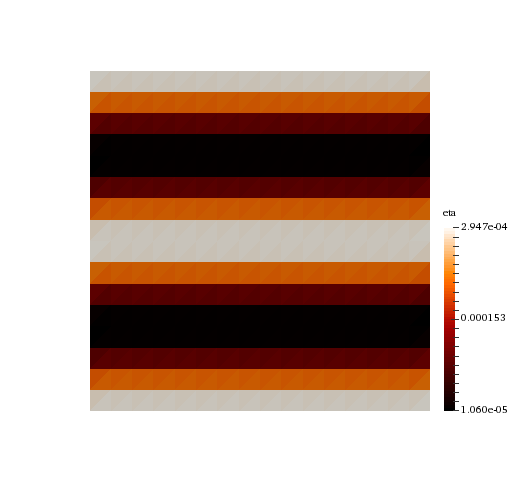
\includegraphics[width=\textwidth,height=\textheight,keepaspectratio,height=\textheight,keepaspectratio]{figures/poisson/P2/eta_16.png}
%    \caption{$N=16$}
%  \end{subfigure}
%  \begin{subfigure}[b]{0.24\textwidth}
%    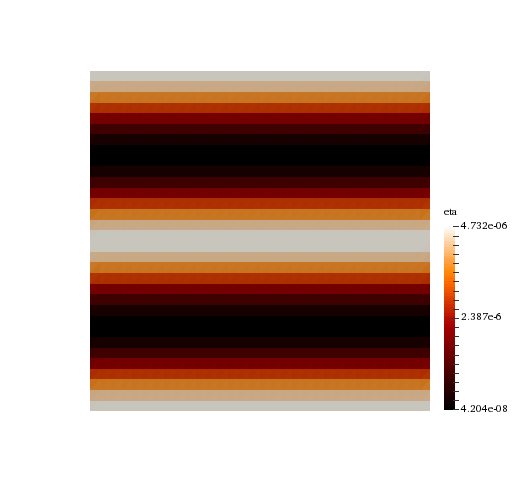
\includegraphics[width=\textwidth,height=\textheight,keepaspectratio,height=\textheight,keepaspectratio]{figures/poisson/P2/eta_32.png}
%    \caption{$N=32$}
%  \end{subfigure}
%  \begin{subfigure}[b]{0.24\textwidth}
%    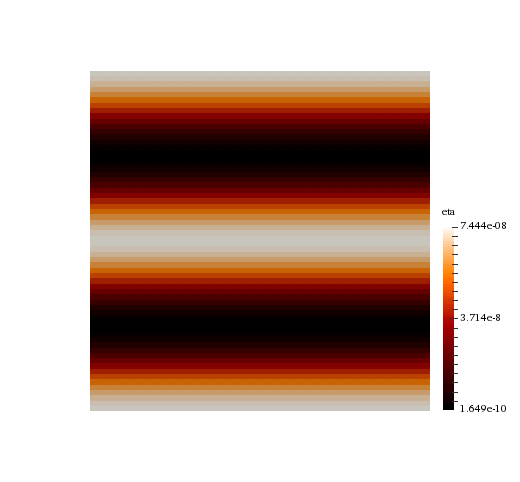
\includegraphics[width=\textwidth,height=\textheight,keepaspectratio,height=\textheight,keepaspectratio]{figures/poisson/P2/eta_64.png}
%    \caption{$N=64$}
%  \end{subfigure}
%  \caption{Error magnitude for $\eta$ for the Poisson model discretized with $P_2$ elements} \label{fig:poisson_eta_P2}
%\end{figure}
%\mbox{}\\
%\begin{figure}[h!]
%  \centering
%  \begin{subfigure}[b]{0.24\textwidth}
%    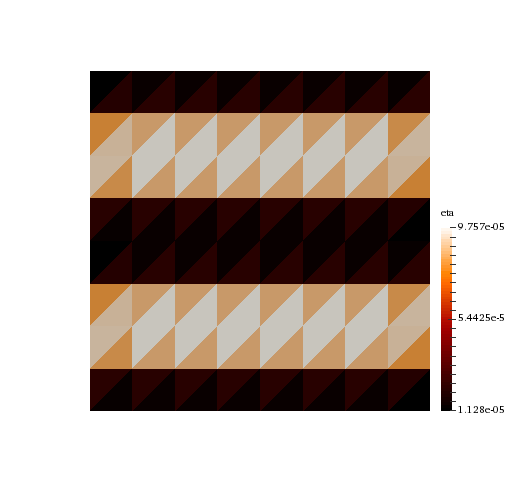
\includegraphics[width=\textwidth,height=\textheight,keepaspectratio,height=\textheight,keepaspectratio]{figures/poisson/P3/eta_8.png}
%    \caption{$N=8$}
%  \end{subfigure}
%  \begin{subfigure}[b]{0.24\textwidth}
%    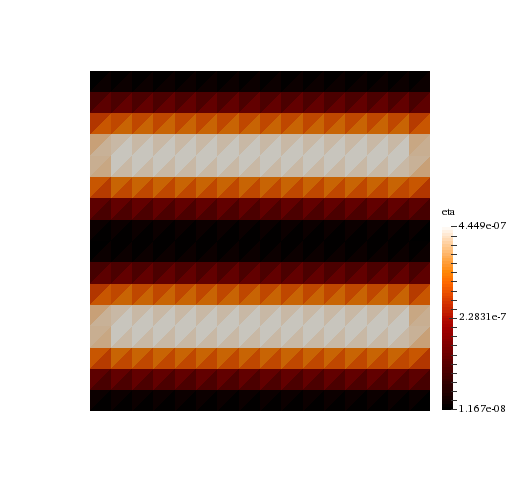
\includegraphics[width=\textwidth,height=\textheight,keepaspectratio,height=\textheight,keepaspectratio]{figures/poisson/P3/eta_16.png}
%    \caption{$N=16$}
%  \end{subfigure}
%  \begin{subfigure}[b]{0.24\textwidth}
%    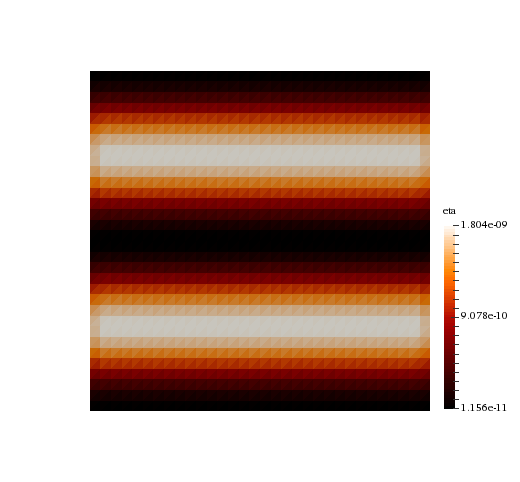
\includegraphics[width=\textwidth,height=\textheight,keepaspectratio,height=\textheight,keepaspectratio]{figures/poisson/P3/eta_32.png}
%    \caption{$N=32$}
%  \end{subfigure}
%  \begin{subfigure}[b]{0.24\textwidth}
%    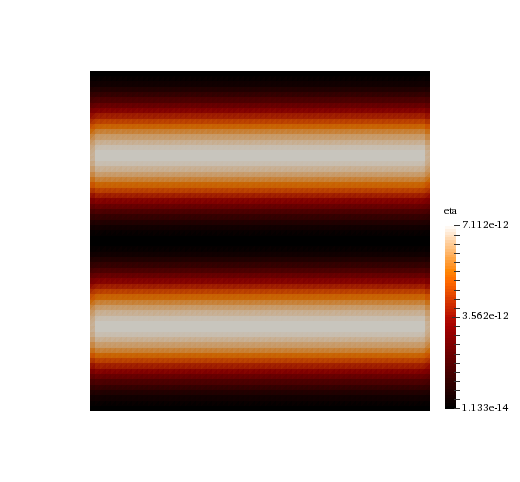
\includegraphics[width=\textwidth,height=\textheight,keepaspectratio,height=\textheight,keepaspectratio]{figures/poisson/P3/eta_64.png}
%    \caption{$N=64$}
%  \end{subfigure}
%  \caption{Error magnitude for $\eta$ for the Poisson model discretized with $P_3$ elements} \label{fig:poisson_eta_P3}
%\end{figure}
\mbox{}\\ \\
\section{Multiple network poroelasticity model (MPET)} \label{section:num_exp_mpet}
This section presents the numerical results from the computation of the a posteriori error estimator derived for the MPET model with a single network (Biot), two networks (Barenblatt-Biot) and a four-network poroelasticity model. The results are validated by computing convergence rates and comparing the results with the theoretical predictions. In addition, the error magnitude for each estimator will be displayed to demonstrate where potential mesh refinement should occur. Note that we will not perform any adaptive mesh refinement in this work. 
\\
\\
To numerically compute the MPET model, we use a manufactured solution and compute the error and convergence rates for the displacement and pressure discretized with Taylor-Hood elements. As we stated in chapter \ref{chap:discretization} we assume Dirichlet boundary conditions, where $u$ and $p$ are equal to some known function on the boundary. In this case, these known functions will be the manufactured solution. 

\subsection{Single network poroelasticity} \label{section:num_exp_mpet1}
In order to evaluate the a posteriori error estimates constructed for the single network poroelasticity model (i.e. the Biot model), we compute their convergence rates under space and time refinement. For the spatial refinement parameter we keep the time step $\tau$ fixed and refine the spatial discretization $h$, and for the temporal refinement, we keep $h$ fixed and refine $\tau$. The manufactured solution chosen for verification for the single network model (Biot) is:
\begin{align*}
u_e = & \, \left(\cos(\pi x)\sin(\pi y)\sin(\pi t), \, \sin(\pi x)\cos(\pi y)\sin(\pi t)\right) \\
p_e = & \, \sin(\pi x) \cos(\pi y)\sin(2\pi t)
\end{align*}
The source terms are found in the same way as described in section \ref{section:mms}. We evaluate the error estimators derived in section \ref{biot:res_err}, which stated that the spatial and temporal error $E$ from section \ref{biot:res_err} could be bounded in the following way,
\begin{equation} \label{biot:error_upbd}
E^n \leq \underbrace{\sup_{m \in [1,N]} (\eta^m_u}_{\eta_1})^\frac{1}{2}  +  \underbrace{(\sum_{m=1}^N \tau_m \eta^m_{p,0})^\frac{1}{2}}_{\eta_2} + \underbrace{\sum_{m=1}^N (\eta^m_u(\delta_t))^\frac{1}{2}}_{\eta_3} + \underbrace{(\sum_{m=1}^N \tau_m \| p_h^m - p_h^{m-1}\|^2_d)^\frac{1}{2}}_{\eta_4}
\end{equation}
\begin{remark}
Note that there are additional terms in $E^n$ other than $\|u - u_{h_{\tau}}\|_{H^1}$ and $\|p - p_{h_{\tau}}\|_{L^2}$. For simplicity, we will only compute these two terms as part of the error to be evaluated. In addition, we have disregarded the data oscillations terms, $\mathcal{E}_{\textnormal{dat}}$ and focused solely on the space and time estimators.
\end{remark}
\mbox{}\\
The a posteriori error estimators indicate how the error behaves in space and time. The space estimator $\eta_1$ is associated with the residual of the displacement $u$, and $\eta_2$ is associated with the residual of the pressure $p$. $\eta_3$ predicts how time may affect the residual of the displacement under space refinement. In other words, $\eta_3$ will indicate how the displacement-residual may change from one time step to the other when we refine in space. Thus, if $\eta_1$ is small compared to $\eta_3$, we should refine in time. Conversely, if $\eta_3$ is small compared to $\eta_1$, we should refine in space. The magnitude of these two estimators indicates \textit{how} to refine. $\eta_4$ is a time estimator associated with the pressure. 
\\
\\
Table \ref{tab:biot_default_space_error} displays the error and convergence rate for the displacement and the pressure under space refinement. We observe that setting all parameters to 1 yields optimal convergence rates for both the displacement and the pressure. The a posteriori error estimators demonstrate optimal order of convergence for $\eta_1$ and $\eta_2$ under space refinement, see table \ref{tab:biot_default_space_est}. Table \ref{tab:biot_default_time_error} presents the error and convergence rate for the displacement and the pressure under space refinement, which yields optimal rates. We also observe optimal rates for the time estimator $\eta_4$ under time refinement, see table \ref{tab:biot_default_time_error}. The error magnitude for the space estimators is illustrated in figures \ref{fig:biot_eta1}, \ref{fig:biot_eta2} and \ref{fig:biot_eta3} for the single network model under space refinement. We observe that the resolution increases as the mesh is refined, which gives an indication where we should concentrate our refinement. The magnitude of $\eta_3$ is much smaller than $\eta_1$, and thus suggests further refinement in space. The error estimators for the displacement and the pressure are different, which gives valuable information regarding how the error for each component behaves under space refinement. That way we can make an informed decision on how to refine, e.g. if we wish to make the solution for $p$ more accurate in space we concentrate the adaptive refinement in the areas indicated by $\eta_2$.
\\
\\
According to the analysis presented in \cite{meunier}, the correct order of convergence for $\eta_3$ should be 2 under space refinement. This is because it is based on the residual of the first equation, which is associated with the displacement. We have already established that we expect second-order convergence for the displacement in the $H^1$-norm when approximated by piecewise quadratics. However, since $\eta_3$ is a time incremental version of $\eta_1$ which is approximated with Backward Euler in time, it may also be reasonable to expect this estimator to converge as a time estimator. %Observing an order lower than expected may be due to errors occurring when we numerically compute the divergence of the stress tensor in FEniCS. 
In addition, we observe that the time estimator $\eta_4$ does not decrease as the mesh is refined, but stays constant. This can be explained by the fact that since it is a time estimator, it may exhibit space-independence when the time step is small compared to the spatial refinement parameter. Figure \ref{fig:biot_eta4} displays the error magnitude for the time estimator $\eta_4$ under time refinement. The lighter areas indicate higher error concentration, which indicates a potential for adaptive refinement. %In order to investigate why we observe incorrect rates, space/time-refinement are presented in tables \ref{tab:biot_default_time_space_eta1}, \ref{tab:biot_default_time_space_eta2}, \ref{tab:biot_default_time_space_eta3}, \ref{tab:biot_default_time_space_eta4} for $\eta_1$, $\eta_2$, $\eta_3$ and $\eta_4$, respectively. \todo{explain space/time tables!}
%%%%%%%%%%%%%%%%%%%%%%%%%%%%%%%%%%%%%%%%%%%%%%%%%%%%%%
\\
\\
\begin{center} 
\centering
\begin{tabular}{c|c|c|c|c}
$h^{-1}$ & $\|u - u_{h_{\tau}}\|_{H^1}$ & Rate & $\|p - p_{h_{\tau}}\|_{L^2}$ & Rate\\\hline
4  & 1.947e-2 & -     & 1.788e-3 & - \\
8  & 4.693e-3 & 2.053 & 6.245e-4 & 1.518 \\
16 & 1.141e-3 & 2.041 & 1.755e-4 & 1.832 \\
32 & 2.835e-4 & 2.008 & 4.313e-5 & 2.024 \\
64 & 7.192e-5 & 1.979 & 1.026e-5 & 2.072 \\\hline
Opt. & & 2 & & 2 
\end{tabular}
\captionof{table}{Error norms and convergence rates for Biot model under space refinement, $T=0.1$, $\tau = 5.0$e-5, $\mu=0.5$, all other parameters set to $1$} \label{tab:biot_default_space_error}
\end{center}
\mbox{}\\ \\
\begin{center} 
\centering
\begin{tabular}{c|c|c|c|c|c|c|c}
$h^{-1}$ & $\eta_1$ & Rate &  $\eta_2$ & Rate & $\eta_3$ & Rate & $\eta_4$\\\hline
4  & 9.015e-1 & -     & 3.621e-1 & -     & 1.509e-3 & -     & 2.027e-4 \\
8  & 2.343e-1 & 1.944 & 2.002e-1 & 0.855 & 7.763e-4 & 0.959 & 2.060e-4 \\
16 & 5.916e-2 & 1.986 &1.034e-1  & 0.954 & 3.913e-4 & 0.988 & 2.066e-4 \\
32 & 1.483e-2 & 1.996 & 5.232e-2 & 0.982 & 1.961e-4 & 0.997 & 2.068e-4 \\
64 & 3.711e-3 & 1.999 & 2.630e-2 & 0.992 & 9.810e-5 & 0.999 & 2.068e-4 \\\hline
Opt. & & 2 & & 1 & & 2\footnote[1]{According to \cite{meunier}, the correct order of convergence for $\eta_3$ should be 2.} & 
\end{tabular}
\captionof{table}{Convergence rate for a posteriori error estimates for the Biot model under space refinement, $T=0.1$, $\tau = 5.0$e-5, $\mu=0.5$, all other parameters set to $1$} \label{tab:biot_default_space_est}

\clearpage
\begin{center}
\centering
\begin{tabular}{c|c|c|c|c}
$\tau$ & $\|u-u_{h_{\tau}}\|_{H^1}$ & Rate & $\|p-p_{h_{\tau}}\|_{L^2}$ & Rate \\\hline
0.02    & 1.392e-3 & -     & 4.184e-3 & -     \\
0.01    & 5.838e-4 & 1.253 & 1.768e-3 & 1.243 \\
0.005   & 2.644e-4 & 1.143 & 8.026e-4 & 1.139 \\
0.0025  & 1.203e-4 & 1.136 & 3.657e-4 & 1.134 \\
0.00125 & 6.079e-5 & 0.985 & 1.828e-4 & 1.000 \\ \hline
Opt. & & 1 & & 1 
\end{tabular}
\captionof{table}{A priori error estimates, a posteriori error estimates and convergence rates for the Biot model under time refinement, $T=1$, $h=1/128$, $\mu=0.5$, all other parameters set to $1$} \label{tab:biot_default_time_error}
\end{center}
\end{center}
\mbox{}\\ \\
\begin{center} 
\centering
\begin{tabular}{c|c|c|c|c|c}
$\tau$ & $\eta_1$ & $\eta_2$ & $\eta_3$ & $\eta_4$ & Rate\\\hline
0.02    & 2.947e-3 & 8.375e-2 & 1.961e-2 & 1.923e-1 & -    \\
0.01    & 2.947e-3 & 8.411e-2 & 9.809e-3 & 9.742e-2 & 0.981\\
0.005   & 2.948e-3 & 8.431e-2 & 4.905e-3 & 4.903e-2 & 0.991\\
0.0025  & 2.948e-3 & 8.441e-2 & 2.453e-3 & 2.466e-2 & 0.992\\
0.00125 & 2.948e-3 & 8.446e-2 & 1.226e-3 & 1.233e-2 & 0.999\\\hline
Opt. & & & & & 1
\end{tabular}
\captionof{table}{Convergence rate for a posteriori error estimates for the Biot model under time refinement, $T=1$, $h=1/128$, $\mu=0.5$, all other parameters set to $1$} \label{tab:biot_default_time_est}
\end{center}
\mbox{}\\ \\
\begin{figure}[h!]
  \centering
  \begin{subfigure}[b]{0.24\textwidth}
    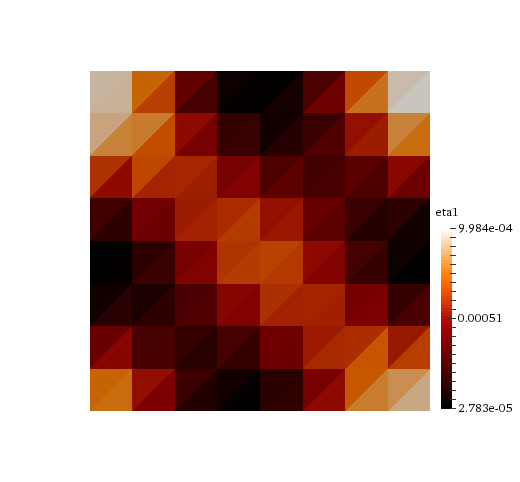
\includegraphics[width=\textwidth,height=\textheight,keepaspectratio,height=\textheight,keepaspectratio]{figures/1_mpet/space/eta1_8.png}
    \caption{$N=8$}
  \end{subfigure}
  \begin{subfigure}[b]{0.24\textwidth}
    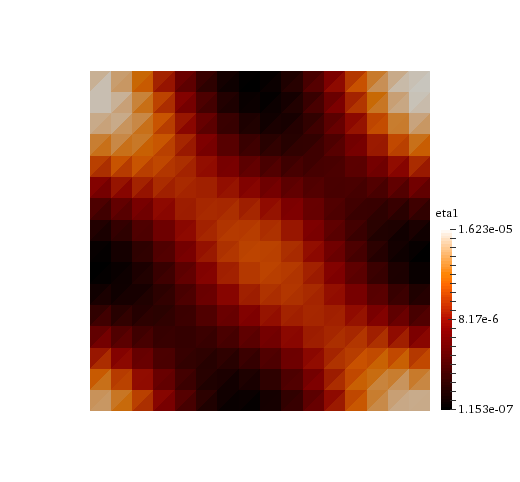
\includegraphics[width=\textwidth,height=\textheight,keepaspectratio,height=\textheight,keepaspectratio]{figures/1_mpet/space/eta1_16.png}
    \caption{$N=16$}
  \end{subfigure}
  \begin{subfigure}[b]{0.24\textwidth}
    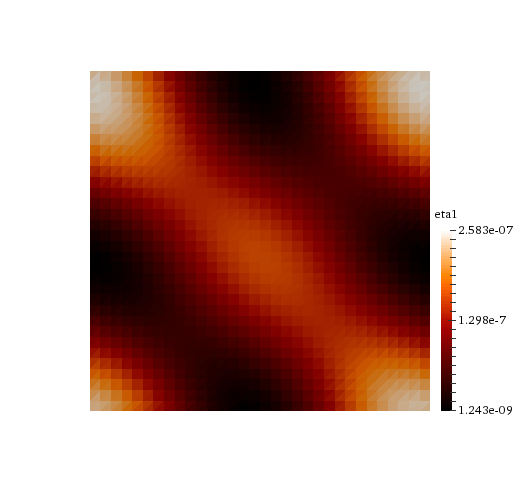
\includegraphics[width=\textwidth,height=\textheight,keepaspectratio,height=\textheight,keepaspectratio]{figures/1_mpet/space/eta1_32.png}
    \caption{$N=32$}
  \end{subfigure}
  \begin{subfigure}[b]{0.24\textwidth}
    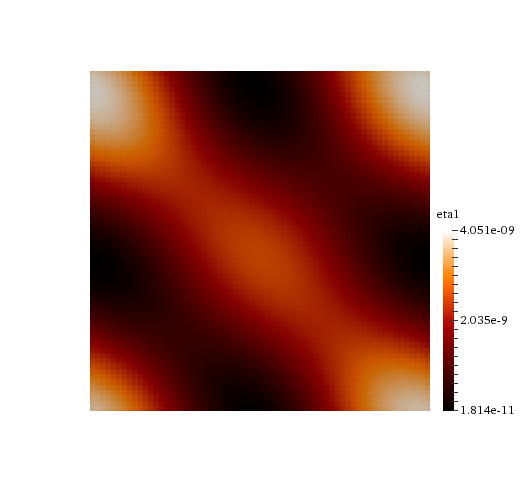
\includegraphics[width=\textwidth,height=\textheight,keepaspectratio,height=\textheight,keepaspectratio]{figures/1_mpet/space/eta1_64.png}
    \caption{$N=64$}
  \end{subfigure}
  \caption{Error magnitude for $\eta_1$ under space refinement at $t=T$ for single network MPET model} \label{fig:biot_eta1}
\end{figure}

\clearpage

\begin{figure}[h!]
  \centering
  \begin{subfigure}[b]{0.24\textwidth}
    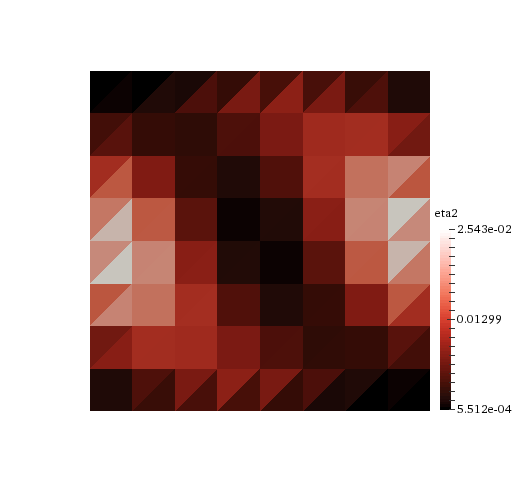
\includegraphics[width=\textwidth,height=\textheight,keepaspectratio,height=\textheight,keepaspectratio]{figures/1_mpet/space/eta2_8.png}
    \caption{$N=8$}
  \end{subfigure}
  \begin{subfigure}[b]{0.24\textwidth}
    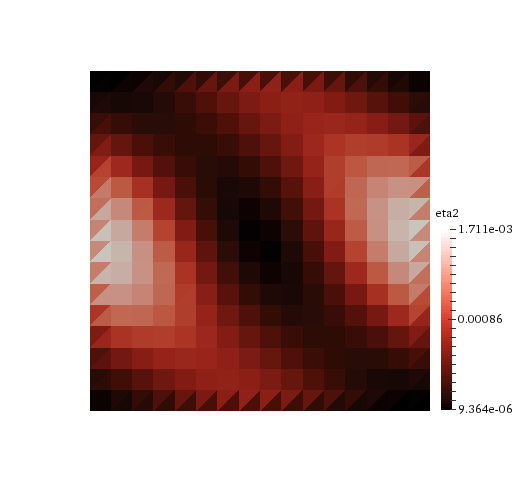
\includegraphics[width=\textwidth,height=\textheight,keepaspectratio,height=\textheight,keepaspectratio]{figures/1_mpet/space/eta2_16.png}
    \caption{$N=16$}
  \end{subfigure}
  \begin{subfigure}[b]{0.24\textwidth}
    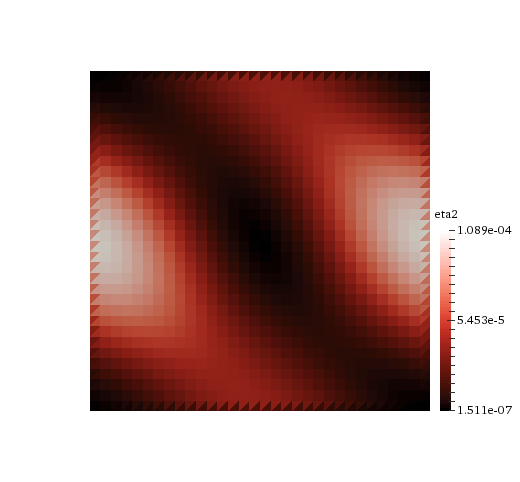
\includegraphics[width=\textwidth,height=\textheight,keepaspectratio,height=\textheight,keepaspectratio]{figures/1_mpet/space/eta2_32.png}
    \caption{$N=32$}
  \end{subfigure}
  \begin{subfigure}[b]{0.24\textwidth}
    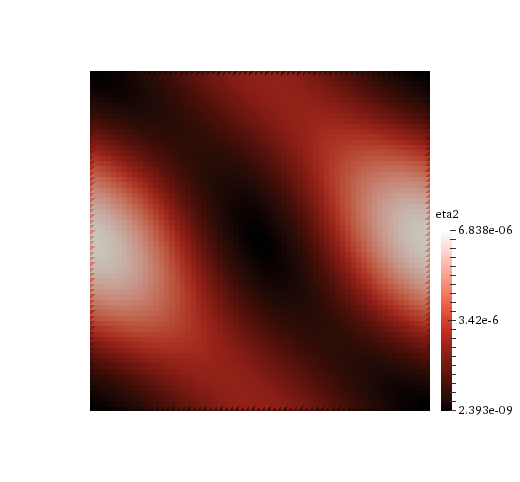
\includegraphics[width=\textwidth,height=\textheight,keepaspectratio,height=\textheight,keepaspectratio]{figures/1_mpet/space/eta2_64.png}
    \caption{$N=64$}
  \end{subfigure}
  \caption{Error magnitude for $\eta_2$ under space refinement at $t=T$ for single network MPET model} \label{fig:biot_eta2}
\end{figure}
\mbox{}\\ \\
\begin{figure}[h!]
  \centering
  \begin{subfigure}[b]{0.24\textwidth}
    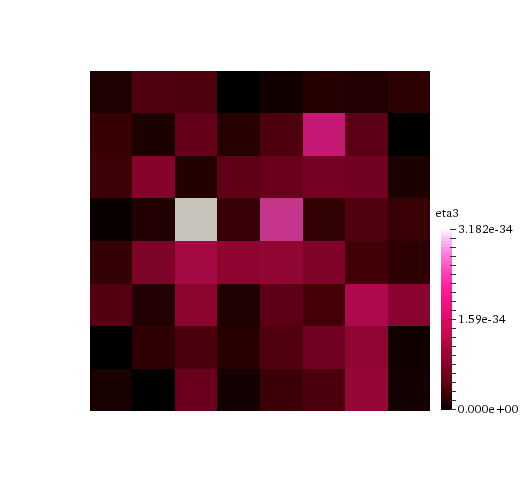
\includegraphics[width=\textwidth,height=\textheight,keepaspectratio,height=\textheight,keepaspectratio]{figures/1_mpet/space/eta3_8.png}
    \caption{$N=8$}
  \end{subfigure}
  \begin{subfigure}[b]{0.24\textwidth}
    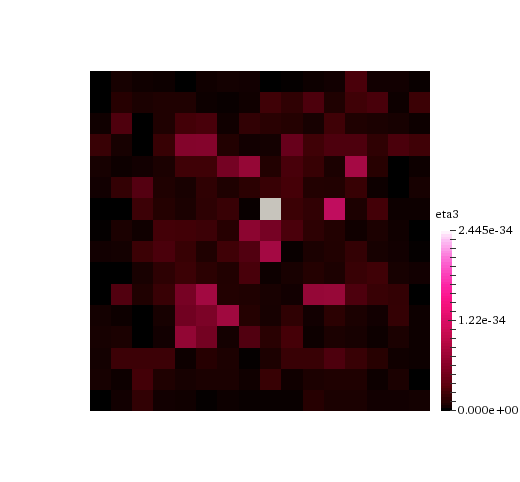
\includegraphics[width=\textwidth,height=\textheight,keepaspectratio,height=\textheight,keepaspectratio]{figures/1_mpet/space/eta3_16.png}
    \caption{$N=16$}
  \end{subfigure}
  \begin{subfigure}[b]{0.24\textwidth}
    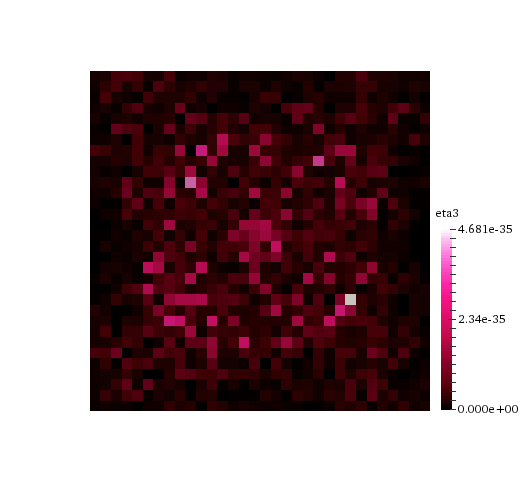
\includegraphics[width=\textwidth,height=\textheight,keepaspectratio,height=\textheight,keepaspectratio]{figures/1_mpet/space/eta3_32.png}
    \caption{$N=32$}
  \end{subfigure}
  \begin{subfigure}[b]{0.24\textwidth}
    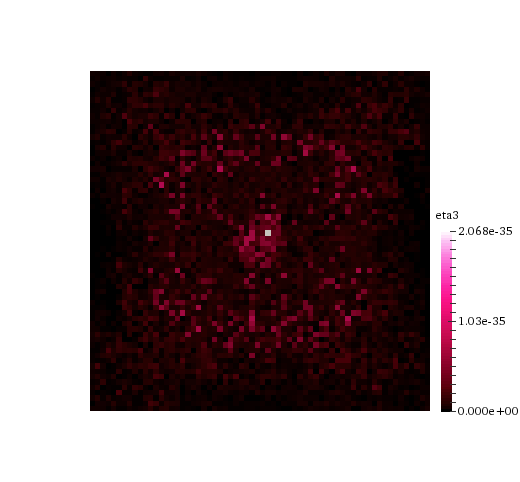
\includegraphics[width=\textwidth,height=\textheight,keepaspectratio,height=\textheight,keepaspectratio]{figures/1_mpet/space/eta3_64.png}
    \caption{$N=64$}
  \end{subfigure}
  \caption{Error magnitude for $\eta_3$ under space refinement at $t=T$ for single network MPET model} \label{fig:biot_eta3}
\end{figure}
\mbox{}\\ \\
\begin{figure}[h!]
  \centering
  \begin{subfigure}[b]{0.24\textwidth}
    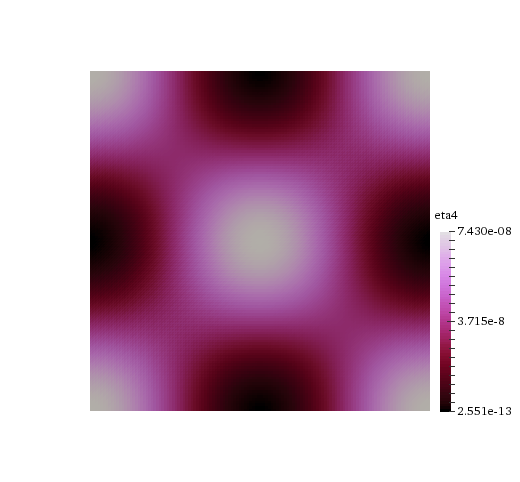
\includegraphics[width=\textwidth,height=\textheight,keepaspectratio,height=\textheight,keepaspectratio]{figures/1_mpet/time/eta4_dt1.png}
    \caption{$\tau=0.01$}
  \end{subfigure}
  \begin{subfigure}[b]{0.24\textwidth}
    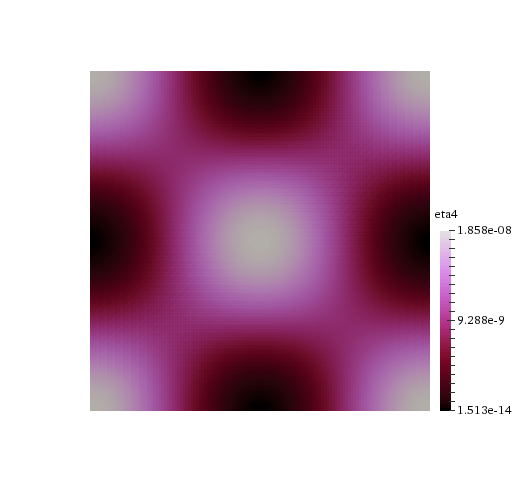
\includegraphics[width=\textwidth,height=\textheight,keepaspectratio,height=\textheight,keepaspectratio]{figures/1_mpet/time/eta4_dt2.png}
    \caption{$\tau=0.005$}
  \end{subfigure}
  \begin{subfigure}[b]{0.24\textwidth}
    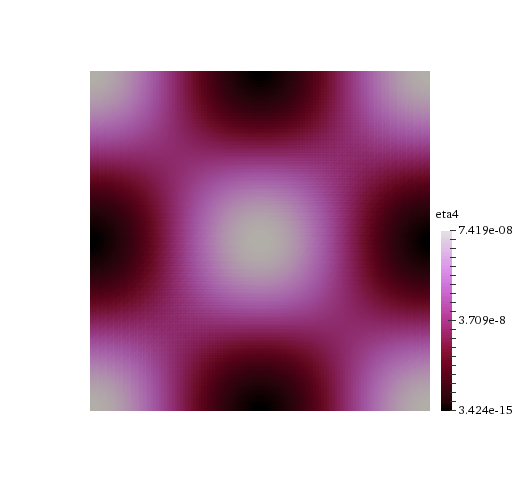
\includegraphics[width=\textwidth,height=\textheight,keepaspectratio,height=\textheight,keepaspectratio]{figures/1_mpet/time/eta4_dt3.png}
    \caption{$\tau=0.0025$}
  \end{subfigure}
  \begin{subfigure}[b]{0.24\textwidth}
    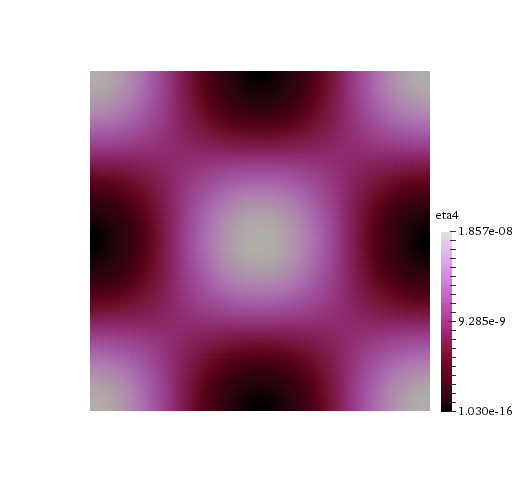
\includegraphics[width=\textwidth,height=\textheight,keepaspectratio,height=\textheight,keepaspectratio]{figures/1_mpet/time/eta4_dt4.png}
    \caption{$\tau=0.00125$}
  \end{subfigure}
  \caption{Error magnitude for $\eta_4$ under time refinement at $t=T$ for single network MPET model} \label{fig:biot_eta4}
\end{figure}
\clearpage
%\begin{center} 
%\centering
%\begin{tabular}{c|c|c|c|c}
%$\tau$ / $h^{-1}$ & 4        & 8        & 16      & 32    \\\hline
%$1/4^2$   & 2.865e+0 & 7.440e-1 & 1.878e-1 & 4.707e-2 \\   
%$1/8^2$   & 2.867e+0 & 7.446e-1 & 1.879e-1 & 4.710e-2 \\
%$1/16^2$  & 2.868e+0 & 7.448e-1 & 1.879e-1 & 4.711e-2 \\
%$1/32^2$  & 2.868e+0 & 7.448e-1 & 1.879e-1 & 4.711e-2 \\
%\end{tabular}
%\captionof{table}{Error estimates for $\eta_1$ under space/time refinement, $T=1$, $\mu=0.5$, all other parameters set to $1$} \label{tab:biot_default_time_space_eta1}
%\end{center}
%\mbox{}\\
%\begin{center} 
%\centering
%\begin{tabular}{c|c|c|c|c}
%$\tau$ / $h^{-1}$ & 4        & 8        & 16      & 32    \\\hline
%$1/4^2$   & 2.216e+0 & 1.243e+0 & 6.465e-1 & 3.279e-1 \\   
%$1/8^2$   & 2.224e+0 & 1.257e+0 & 6.553e-1 & 3.327e-1 \\
%$1/16^2$  & 2.230e+0 & 1.262e+0 & 6.586e-1 & 3.344e-1 \\
%$1/32^2$  & 2.231e+0 & 1.263e+0 & 6.594e-1 & 3.349e-1 \\
%\end{tabular}
%\captionof{table}{Error estimates for $\eta_2$ under space/time refinement, $T=1$, $\mu=0.5$, all other parameters set to $1$} \label{tab:biot_default_time_space_eta2}
%\end{center}
%\mbox{}\\
%\begin{center} 
%\centering
%\begin{tabular}{c|c|c|c|c}
%$\tau$ / $h^{-1}$ & 4 & 8 & 16 & 32    \\\hline
%$1/4^2$  & 1.873e+0 & 9.637e-1 & 4.858e-1 & 2.434e-1 \\   
%$1/8^2$  & 4.714e-1 & 2.425e-1 & 1.222e-1 & 6.125e-2 \\
%$1/16^2$ & 1.179e-1 & 6.064e-2 & 3.057e-2 & 1.532e-2 \\
%$1/32^2$ & 2.948e-2 & 1.516e-2 & 7.643e-3 & 3.830e-3 \\
%\end{tabular}
%\captionof{table}{Error estimates for $\eta_3$ under space/time refinement, $T=1$, $\mu=0.5$, all other parameters set to $1$} \label{tab:biot_default_time_space_eta3}
%\end{center}
%\mbox{}\\
%\begin{center}
%\centering
%\begin{tabular}{c|c|c|c|c}
%$\tau$ / $h^{-1}$ & 4        & 8        & 16      & 32    \\\hline
%$1/4^2$   & 5.881e-1 & 5.999e-1 & 6.029e-1 & 6.037e-1 \\   
%$1/8^2$   & 1.489e-1 & 1.523e-1 & 1.532e-1 & 1.534e-1 \\
%$1/16^2$  & 3.730e-2 & 3.820e-2 & 3.843e-2 & 3.849e-2 \\
%$1/32^2$  & 9.331e-3 & 9.556e-3 & 9.616e-3 & 9.631e-3 \\
%\end{tabular}
%\captionof{table}{Error estimates for $\eta_4$ under space/time refinement, $T=1$, $\mu=0.5$, all other parameters set to $1$}  \label{tab:biot_default_time_space_eta4}
%\end{center}

\subsection{Two-network poroelasticity} \label{test_bb}
For the two-network poroelasticity model (Barenblatt-Biot) we use the following manufactured solution,
\begin{align*}
u_e = & \, \left(\cos(\pi x)\sin(\pi y)\sin(\pi t), \, \sin( \pi x)\cos(\pi y)\sin(\pi t)\right) \\
p_{1_e} = & \,\sin(\pi x) \cos(\pi y)\sin(2\pi t)  \\
p_{2_e} = & \,\cos(\pi x) \sin(\pi y)\sin(2\pi t)
\end{align*}
This section presents the numerical results obtained from computing the a posteriori error estimates constructed for the two-network poroelasticity model (i.e. the Barenblatt-Biot model) in section  \ref{section:error_bb}. The results include both a spatial and temporal refinement, with the same discretization parameters as for the single network model. The estimators have been implemented using the test problem described in section \ref{test_bb} using Taylor-Hood elements.
\\
\\
We use the error estimators derived in section \ref{bb:case1_res_err}, which stated that the spatial and temporal error $E$ from \eqref{bb:error} could be bounded in the following way,
\begin{align} 
E^n \leq & \underbrace{\sup_{m \in [1,N]} (\eta^m_u)^\frac{1}{2}}_{\eta_1} + \underbrace{\left(\sum_{m=1}^N \tau_m \eta^m_{p_1,0} + \eta^m_{p_2,0}\right)^\frac{1}{2}}_{\eta_2} + \underbrace{\sum_{m=1}^N (\eta^m_u(\delta_t))^\frac{1}{2}}_{\eta_3} \\
& + \underbrace{\left(\sum_{m=1}^N \tau_m (\|p^m_{1h} - p^{m-1}_{1h}\|_d^2 + \|p^m_{2h} - p^{m-1}_{2h}\|_d^2) )\right)^\frac{1}{2}}_{\eta_4}
\end{align}
\begin{remark}
Note that there are additional terms in $E^n$ other than $\|u - u_{h_{\tau}}\|_{H^1}$, $\|p_1 - p_{1h_{\tau}}\|_{L^2}$ and $\|p_2 - p_{2h_{\tau}}\|_{L^2}$. For simplicity, we will only compute these two terms as part of the error to be evaluated. In addition, we have disregarded the data oscillations terms, $\mathcal{E}_{\textnormal{dat}}$ and focused solely on the space and time estimators for the numerical experiments.
\end{remark}
\mbox{}\\
The a posteriori error estimators indicate how the error behaves in space and time. The space estimator $\eta_1$ is associated with the residual of the displacement $u$, and $\eta_2$ is associated with the residual of the pressures $p_1$ and $p_2$. $\eta_3$ predicts how time may affect the residual of the displacement under space refinement. The magnitude of these two estimators gives an indication of \textit{how} to refine. $\eta_4$ is a time estimator associated with the pressure. 
\\
\\
The first experiment is implemented assuming non-interacting fluid networks, with $\mu = 0.5$, $\xi_1 = \xi_2 = 0$ and all other parameters to $1$. The same experiment is then executed with interacting fluid networks. Additionally, an experiment with physiologically inspired parameters is presented.  
\\
\subsubsection{Two-network poroelasticity: non-interacting fluid networks}
Table \ref{tab:bb_no_transfer_space_error} present the convergence rates for the a priori error estimate for the displacement and the pressures under space refinement with non-interacting fluid networks. The displacement and the pressure converge optimally as the mesh is refined. We observe that the a posteriori error estimators yields the same rates as for the Biot model, where we see one order lower for $\eta_3$ than what is expected according to \cite{meunier}, see table \ref{tab:bb_no_transfer_space_est}. The quantity $\eta_4$, which is associated with the time error remains constant under space refinement. Figures \ref{fig:bb_no_transfer_eta1}, \ref{fig:bb_no_transfer_eta2} and \ref{fig:bb_no_transfer_eta3} present the error magnitude for the space estimators for the two-network model under space refinement. Similarly, as with the single network model, the magnitude for $\eta_3$ is much smaller than $\eta_1$ indicating further space refinement, and not time refinement. Recall that $\eta_3$ is a space estimator predicting the effect of time on the displacement under space refinement. Thus, when this quantity is much smaller than the space estimator for the displacement suggests adaptive refinement in space. The quantity $\eta_1$ predicts how the spatial error for $u$ will behave, while $\eta_2$ predicts the behavior of the spatial error for the pressures $p_1$ and $p_2$.
\\
\\
Table \ref{tab:bb_no_transfer_time_error} displays the convergence rate for the a priori error estimate for the displacement and the pressures under time refinement with non-interacting fluid networks. The displacement and the pressure exhibit optimal convergence as the time step is refined. Running simulations with smaller time steps ensure convergence of order 1. The time estimator $\eta_4$ converges optimally, see table \ref{tab:bb_no_transfer_time_est}. Figure \ref{fig:bb_no_transfer_eta4} displays the time estimator $\eta_4$ under time refinement. We observe that the overall accuracy of the error increases under time refinement. The lighter areas indicate a higher error, which suggests a potential adaptive refinement to be concentrated here. 
\\
\\
\begin{center} 
\centering
\begin{tabular}{c|c|c|c|c|c|c}
$h^{-1}$ & $\|u - u_{h_{\tau}}\|_{H^1}$ & Rate & $\|p_1 - p_{1h_{\tau}}\|_{L^2}$ & Rate & $\|p_2 - p_{2h_{\tau}}\|_{L^2}$ & Rate\\\hline
4  & 3.458e-2 & -     & 1.999e-3 & -     & 1.999e-3 & - \\
8  & 8.318e-3 & 2.055 & 9.255e-4 & 1.111 & 9.255e-4 & 1.111 \\
16 & 2.038e-3 & 2.029 & 2.641e-4 & 1.809 & 2.641e-4 & 1.809 \\
32 & 5.081e-4 & 2.004 & 6.615e-5 & 1.997 & 6.615e-5 & 1.997 \\
64 & 1.286e-4 & 1.982 & 1.543e-5 & 2.100 & 1.543e-5 & 2.100 \\\hline
Opt. & & 2 & & 2 & & 2
\end{tabular}
\captionof{table}{Error norms and convergence rates for Barenblatt-Biot model with non-interacting fluid networks under space refinement, $T=0.1$, $\tau = 5.0$e-5, $\mu=0.5$, $\xi_1 = \xi_2 = 0$, all other parameters set to $1$} \label{tab:bb_no_transfer_space_error}
\end{center}

\clearpage

\begin{center} 
\centering
\begin{tabular}{c|c|c|c|c|c|c|c}
$h^{-1}$ & $\eta_1$ & Rate &  $\eta_2$ & Rate & $\eta_3$ & Rate & $\eta_4$\\\hline
4  & 9.626e-1 & -     & 5.172e-1 & -     & 1.530e-3 & -     & 2.875e-4 \\
8  & 2.454e-1 & 1.972 & 2.839e-1 & 0.865 & 7.860e-4 & 0.961 & 2.915e-4 \\
16 & 6.167e-2 & 1.992 & 1.462e-1 & 0.958 & 3.961e-4 & 0.988 & 2.922e-4 \\
32 & 1.544e-2 & 1.998 & 7.396e-2 & 0.983 & 1.985e-4 & 0.997 & 2.924e-4 \\
64 & 3.863e-3 & 1.999 & 3.717e-2 & 0.993 & 9.930e-5 & 0.999 & 2.924e-4 \\\hline
Opt. & & 2 & & 1  & & 2 & 
\end{tabular}
\captionof{table}{Convergence rate for a posteriori error estimates for the Barenblatt-Biot model with non-interacting fluid networks under space refinement, $T=0.1$, $\tau = 5.0$e-5, $\mu=0.5$, $\xi_1 = \xi_2 = 0$, all other parameters set to $1$} \label{tab:bb_no_transfer_space_est}
\end{center}
\mbox{}\\ \\ \\
\begin{center} 
\centering
\small
\begin{tabular}{c|c|c|c|c|c|c}
$\tau$ & $\|u-u_{h_{\tau}}\|_{H^1}$ & Rate & $\|p_1-p_{1h_{\tau}}\|_{L^2}$ & Rate & $\|p_2-p_{2h_{\tau}}\|_{L^2}$ & Rate \\\hline
0.02   	& 2.912e-3 & -     & 4.508e-3 & -     & 4.508e-3 &  -    \\
0.01   	& 1.258e-3 & 1.210 & 1.938e-3 & 1.218 & 1.938e-3 & 1.218 \\
0.005  	& 5.807e-4 & 1.116 & 8.900e-4 & 1.123 & 8.900e-4 & 1.123 \\
0.0025  & 2.798e-4 & 1.053 & 4.261e-4 & 1.062 & 4.261e-4 & 1.062 \\
0.00125 & 1.392e-4 & 1.007 & 2.095e-4 & 1.025 & 2.095e-4 & 1.025 \\ \hline
Opt. & & 1 & & 1  & & 1
\end{tabular}
\normalsize
\captionof{table}{Error estimates and convergence rates for the Barenblatt-Biot model with non-interacting fluid networks under time refinement, $T=1$, $h=1/128$, $\mu=0.5$, $\xi_1 = \xi_2 = 0$, all other parameters set to $1$} \label{tab:bb_no_transfer_time_error}
\end{center}
\mbox{}\\ \\ \\
\begin{center} 
\centering
\begin{tabular}{c|c|c|c|c|c}
$\tau$ & $\eta_1$ & $\eta_2$ & $\eta_3$ & $\eta_4$ & Rate\\\hline
0.02    & 2.948e-3 & 1.185e-1 & 1.985e-2 & 2.719e-1 & -    \\
0.01    & 2.947e-3 & 1.190e-1 & 9.930e-3 & 1.378e-1 & 0.981\\
0.005   & 2.947e-3 & 1.192e-1 & 4.965e-3 & 6.934e-2 & 0.991\\
0.0025  & 2.948e-3 & 1.194e-1 & 2.483e-3 & 3.478e-2 & 0.992\\
0.00125 & 2.948e-3 & 1.194e-1 & 1.241e-3 & 1.742e-2 & 0.998\\\hline
Opt. & & & & & 1
\end{tabular}
\captionof{table}{A posteriori error and convergence rates for the Barenblatt-Biot model with non-interacting fluid networks under time refinement, $T=1$, $h=1/128$, $\mu=0.5$, $\xi_1 = \xi_2 = 0$, all other parameters set to $1$} \label{tab:bb_no_transfer_time_est}
\end{center}

\begin{figure}[h!]
  \centering
  \begin{subfigure}[b]{0.24\textwidth}
    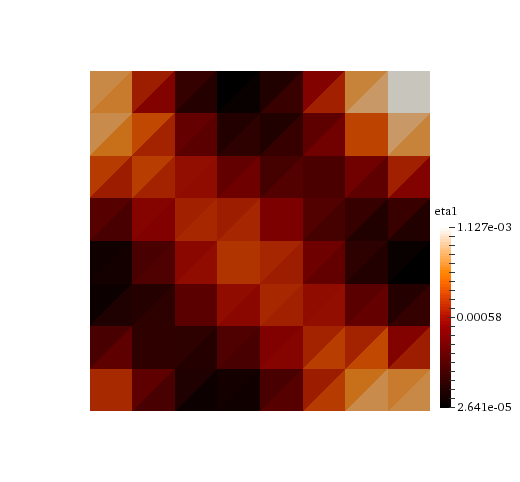
\includegraphics[width=\textwidth,height=\textheight,keepaspectratio,height=\textheight,keepaspectratio]{figures/2_mpet/no_transfer/space/eta1_8.png}
    \caption{$N=8$}
  \end{subfigure}
  \begin{subfigure}[b]{0.24\textwidth}
    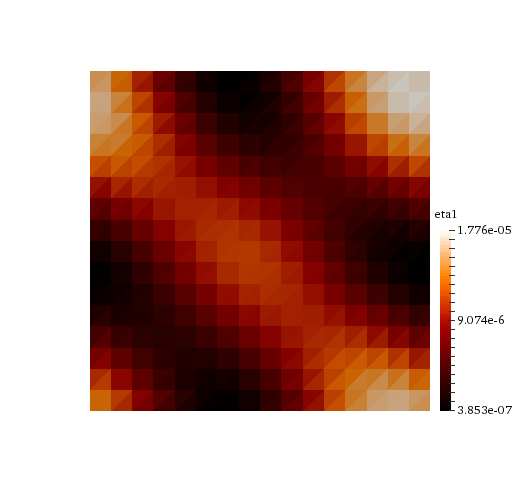
\includegraphics[width=\textwidth,height=\textheight,keepaspectratio,height=\textheight,keepaspectratio]{figures/2_mpet/no_transfer/space/eta1_16.png}
    \caption{$N=16$}
  \end{subfigure}
  \begin{subfigure}[b]{0.24\textwidth}
    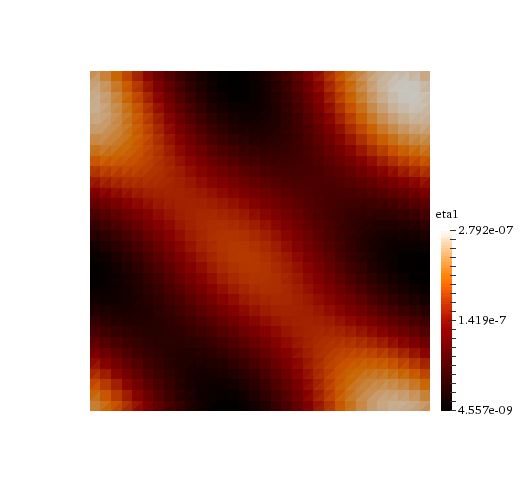
\includegraphics[width=\textwidth,height=\textheight,keepaspectratio,height=\textheight,keepaspectratio]{figures/2_mpet/no_transfer/space/eta1_32.png}
    \caption{$N=32$}
  \end{subfigure}
  \begin{subfigure}[b]{0.24\textwidth}
    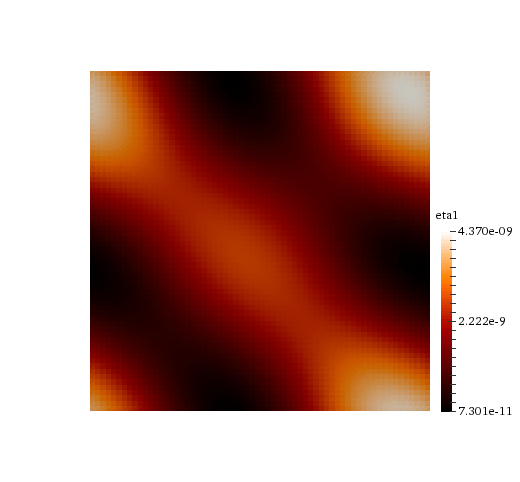
\includegraphics[width=\textwidth,height=\textheight,keepaspectratio,height=\textheight,keepaspectratio]{figures/2_mpet/no_transfer/space/eta1_64.png}
    \caption{$N=64$}
  \end{subfigure}
  \caption{Error magnitude for $\eta_1$ under space refinement at $t=T$ for two-network MPET model with non-interacting fluid networks} \label{fig:bb_no_transfer_eta1}
\end{figure}
\begin{figure}[h!]
  \centering
  \begin{subfigure}[b]{0.24\textwidth}
    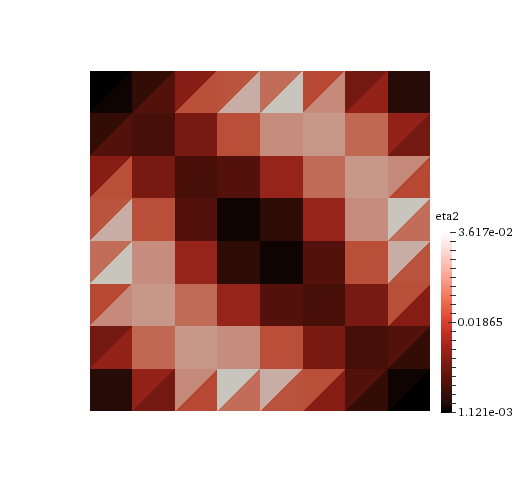
\includegraphics[width=\textwidth,height=\textheight,keepaspectratio,height=\textheight,keepaspectratio]{figures/2_mpet/no_transfer/space/eta2_8.png}
    \caption{$N=8$}
  \end{subfigure}
  \begin{subfigure}[b]{0.24\textwidth}
    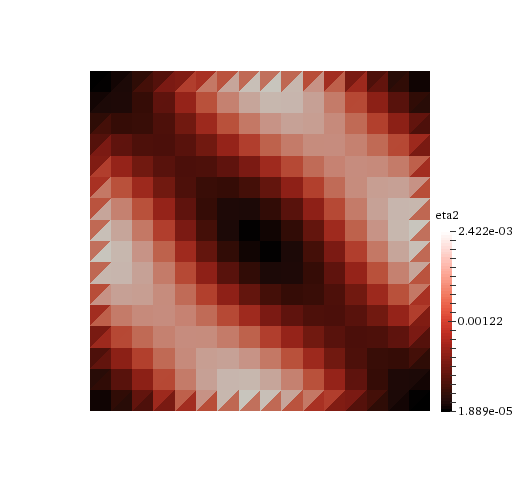
\includegraphics[width=\textwidth,height=\textheight,keepaspectratio,height=\textheight,keepaspectratio]{figures/2_mpet/no_transfer/space/eta2_16.png}
    \caption{$N=16$}
  \end{subfigure}
  \begin{subfigure}[b]{0.24\textwidth}
    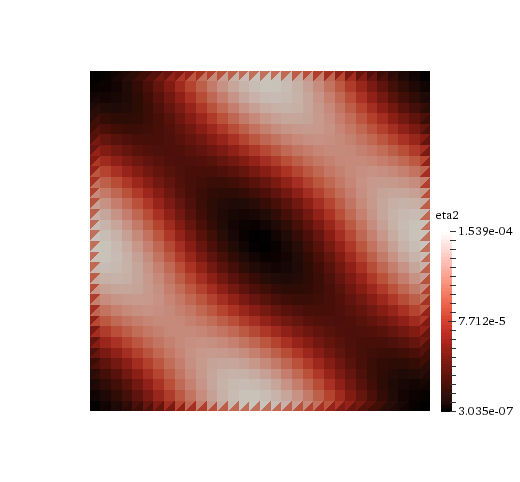
\includegraphics[width=\textwidth,height=\textheight,keepaspectratio,height=\textheight,keepaspectratio]{figures/2_mpet/no_transfer/space/eta2_32.png}
    \caption{$N=32$}
  \end{subfigure}
  \begin{subfigure}[b]{0.24\textwidth}
    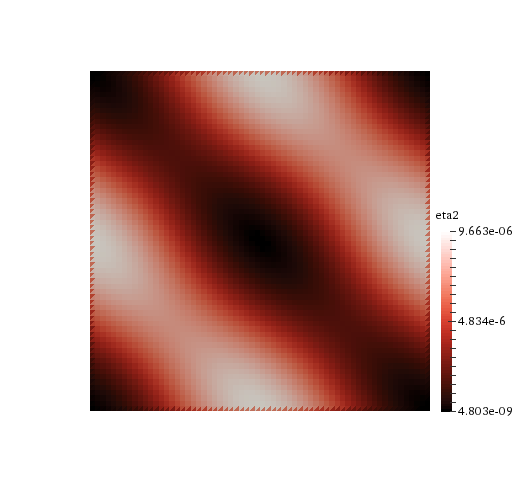
\includegraphics[width=\textwidth,height=\textheight,keepaspectratio,height=\textheight,keepaspectratio]{figures/2_mpet/no_transfer/space/eta2_64.png}
    \caption{$N=64$}
  \end{subfigure}
  \caption{Error magnitude for $\eta_2$ under space refinement at $t=T$ for two-network MPET model with non-interacting fluid networks} \label{fig:bb_no_transfer_eta2}
\end{figure}
\begin{figure}[h!]
  \centering
  \begin{subfigure}[b]{0.24\textwidth}
    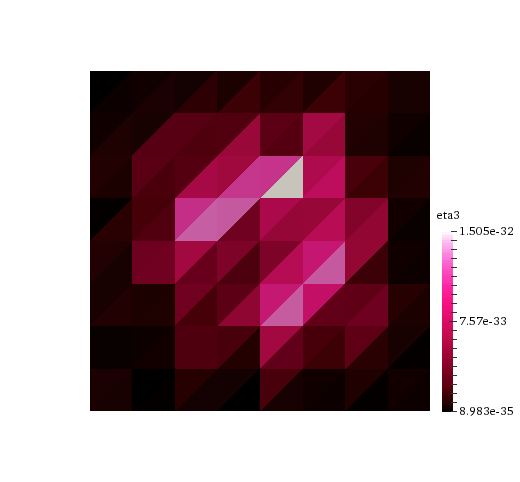
\includegraphics[width=\textwidth,height=\textheight,keepaspectratio,height=\textheight,keepaspectratio]{figures/2_mpet/no_transfer/space/eta3_8.png}
    \caption{$N=8$}
  \end{subfigure}
  \begin{subfigure}[b]{0.24\textwidth}
    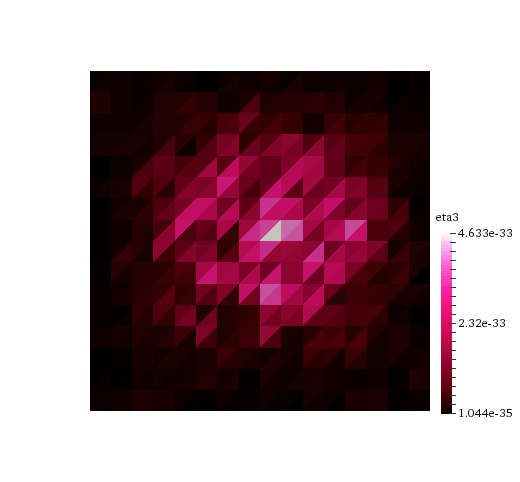
\includegraphics[width=\textwidth,height=\textheight,keepaspectratio,height=\textheight,keepaspectratio]{figures/2_mpet/no_transfer/space/eta3_16.png}
    \caption{$N=16$}
  \end{subfigure}
  \begin{subfigure}[b]{0.24\textwidth}
    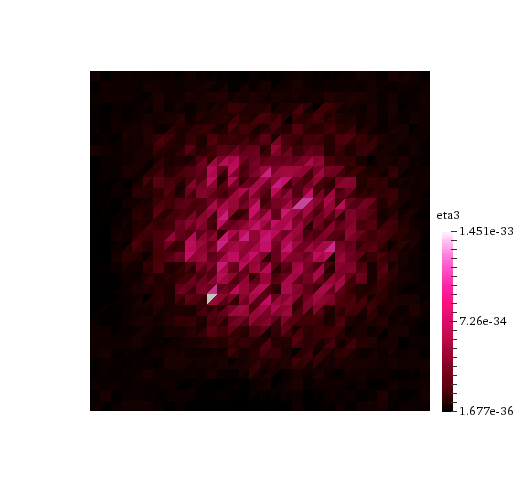
\includegraphics[width=\textwidth,height=\textheight,keepaspectratio,height=\textheight,keepaspectratio]{figures/2_mpet/no_transfer/space/eta3_32.png}
    \caption{$N=32$}
  \end{subfigure}
  \begin{subfigure}[b]{0.24\textwidth}
    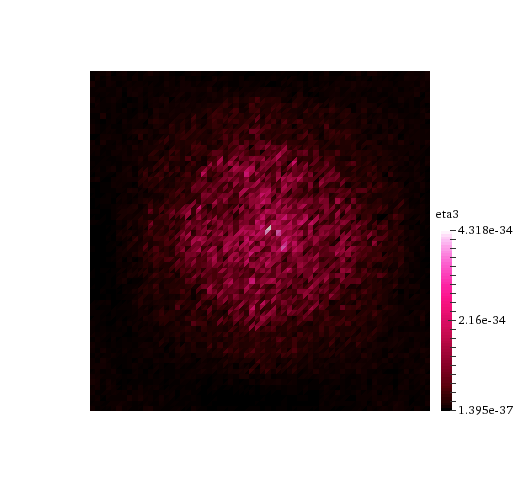
\includegraphics[width=\textwidth,height=\textheight,keepaspectratio,height=\textheight,keepaspectratio]{figures/2_mpet/no_transfer/space/eta3_64.png}
    \caption{$N=64$}
  \end{subfigure}
  \caption{Error magnitude for $\eta_3$ under space refinement at $t=T$ for two-network MPET model with non-interacting fluid networks} \label{fig:bb_no_transfer_eta3}
\end{figure}
\begin{figure}[h!]
  \centering
  \begin{subfigure}[b]{0.24\textwidth}
    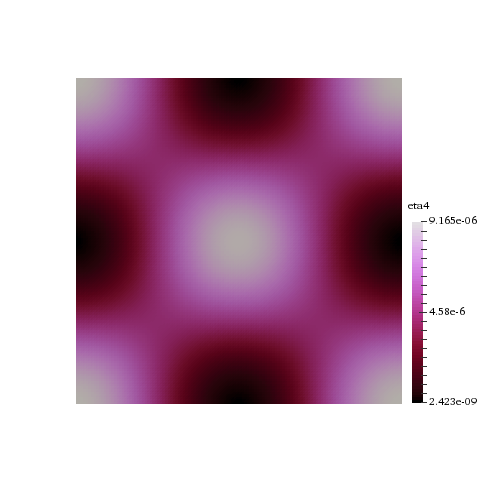
\includegraphics[width=\textwidth,height=\textheight,keepaspectratio,height=\textheight,keepaspectratio]{figures/2_mpet/no_transfer/time/eta4_dt1.png}
    \caption{$\tau=0.01$}
  \end{subfigure}
  \begin{subfigure}[b]{0.24\textwidth}
    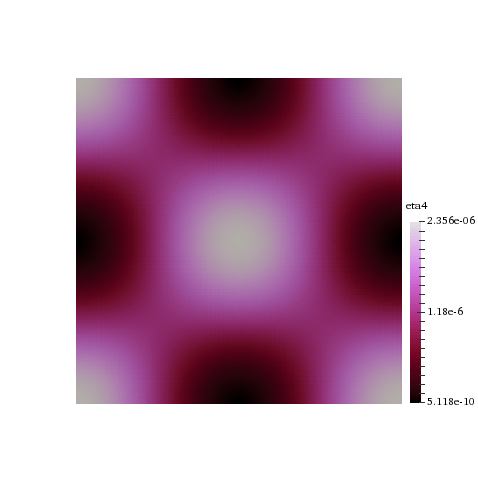
\includegraphics[width=\textwidth,height=\textheight,keepaspectratio,height=\textheight,keepaspectratio]{figures/2_mpet/no_transfer/time/eta4_dt2.png}
    \caption{$\tau=0.005$}
  \end{subfigure}
  \begin{subfigure}[b]{0.24\textwidth}
    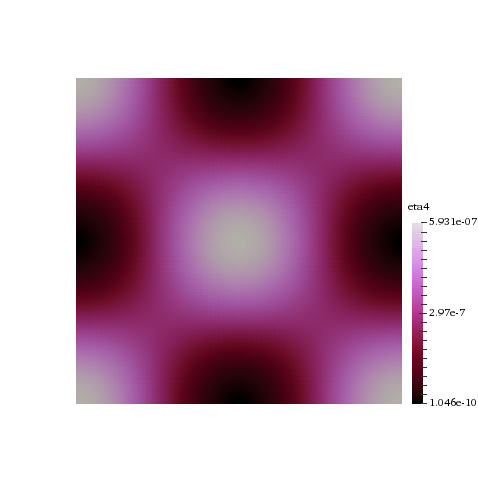
\includegraphics[width=\textwidth,height=\textheight,keepaspectratio,height=\textheight,keepaspectratio]{figures/2_mpet/no_transfer/time/eta4_dt3.png}
    \caption{$\tau=0.0025$}
  \end{subfigure}
  \begin{subfigure}[b]{0.24\textwidth}
    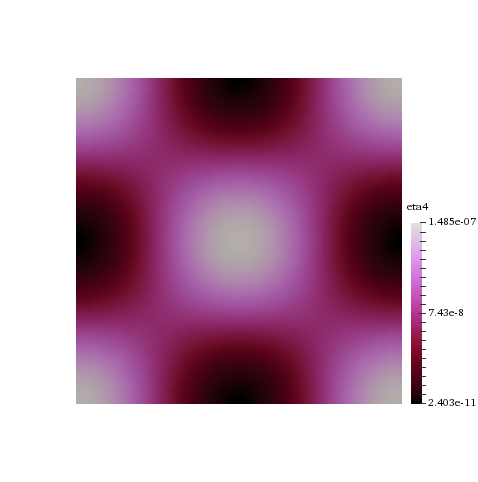
\includegraphics[width=\textwidth,height=\textheight,keepaspectratio,height=\textheight,keepaspectratio]{figures/2_mpet/no_transfer/time/eta4_dt4.png}
    \caption{$\tau=0.00125$}
  \end{subfigure}
  \caption{Error magnitude for $\eta_4$ under time refinement at $t=T$ for two-network MPET model with non-interacting fluid networks} \label{fig:bb_no_transfer_eta4}
\end{figure}
\clearpage
\subsubsection{Two-network poroelasticity: interacting fluid networks} \label{section:num_mpet2_default}
Table \ref{tab:bb_default_transfer_space_error} present the convergence rates for the a priori error estimate for the displacement and the pressures under space refinement with interacting fluid networks where both transfer coefficients are set to 1. The displacement and pressure converge optimally as the mesh is refined. The displacement exhibit the same behavior as with non-interacting fluid networks. This is expected since the displacement is independent of the number of fluid networks. We observe that the a posteriori error estimators yield the same rates as for the Biot model, see table \ref{tab:bb_default_transfer_space_est}. The time estimator $\eta_4$ remains constant under space refinement. The error magnitude for the space estimators $\eta_1$, $\eta_2$ and $\eta_3$ are displayed in figures \ref{fig:bb_default_eta1}, \ref{fig:bb_default_eta2} and \ref{fig:bb_default_eta3}. We observe similar results as with the two network model with non-interacting networks, which indicate that the added transfer terms ($\xi = 1$) do not affect the error magnitude in a significant way.
\\
\\
Table \ref{tab:bb_default_transfer_time_error} displays the convergence rate for the a priori error estimate for the displacement and the pressures under time refinement with interacting fluid networks.  The displacement and the pressure exhibit optimal convergence as the time step is refined. Running simulations with smaller time steps ensure convergence of order 1. The time estimator $\eta_4$ converges optimally, see table \ref{tab:bb_default_transfer_time_est}. Figure \ref{fig:bb_default_eta4} displays the error magnitude for the time estimator $\eta_4$ which is unchanging from the experiment with non-interacting fluid networks. 
\\
\\
\begin{center} 
\centering
\begin{tabular}{c|c|c|c|c|c|c}
$h^{-1}$ & $\|u - u_{h_{\tau}}\|_{H^1}$ & Rate & $\|p_1 - p_{1h_{\tau}}\|_{L^2}$ & Rate & $\|p_2 - p_{2h_{\tau}}\|_{L^2}$ & Rate\\\hline
4  & 3.458e-2 & -     & 2.121e-3 & -     & 2.121e-3 & -     \\
8  & 8.318e-3 & 2.055 & 9.499e-4 & 1.159 & 9.499e-4 & 1.159 \\
16 & 2.038e-3 & 2.029 & 2.699e-4 & 1.816 & 2.699e-4 & 1.816 \\
32 & 5.081e-4 & 2.004 & 6.752e-5 & 1.999 & 6.752e-5 & 1.999 \\
64 & 1.286e-4 & 1.982 & 1.570e-5 & 2.105 & 1.570e-5 & 2.105 \\\hline
Opt. & & 2 & & 2 & & 2
\end{tabular}
\captionof{table}{Error norms and convergence rates for two network MPET model with interacting fluid networks under space refinement, $T=0.1$, $\tau = 5.0$e-5, $\mu=0.5$, $\xi_1 = \xi_2 = 1$, all other parameters set to $1$} \label{tab:bb_default_transfer_space_error}
\end{center}
\mbox{}\\
\begin{center} 
\centering
\begin{tabular}{c|c|c|c|c|c|c|c}
$h^{-1}$ & $\eta_1$ & Rate &  $\eta_2$ & Rate & $\eta_3$ & Rate & $\eta_4$ \\\hline
4  & 9.626e-1 & -     & 5.173e-1 & -     & 1.530e-3 & -     & 4.067e-4 \\
8  & 2.454e-1 & 1.972 & 2.839e-1 & 0.865 & 7.860e-4 & 0.961 & 4.123e-4 \\
16 & 6.167e-2 & 1.992 & 1.462e-1 & 0.958 & 3.961e-4 & 0.988 & 4.133e-4 \\
32 & 1.544e-2 & 1.998 & 7.396e-2 & 0.983 & 1.985e-4 & 0.997 & 4.135e-4 \\
64 & 3.863e-3 & 1.999 & 3.717e-2 & 0.993 & 9.930e-5 & 0.999 & 4.136e-4 \\\hline
Opt. & & 2 & & 1  & & 2 & 
\end{tabular}
\captionof{table}{Convergence rate for a posteriori error estimates for the two network MPET model with interacting fluid networks under space refinement, $T=0.1$, $\tau = 5.0$e-5, $\mu=0.5$, $\xi_1 = \xi_2 = 1$, all other parameters set to $1$} \label{tab:bb_default_transfer_space_est}
\end{center}

\clearpage

\begin{center} 
\centering
\small
\begin{tabular}{c|c|c|c|c|c|c}
$\tau$ & $\|u-u_{h_{\tau}}\|_{H^1}$ & Rate & $\|p_1-p_{1h_{\tau}}\|_{L^2}$ & Rate & $\|p_2-p_{2h_{\tau}}\|_{L^2}$ & Rate \\\hline
0.02   	& 2.912e-3 & -     & 4.503e-3 & -     & 4.503e-3 &  -    \\
0.01   	& 1.258e-3 & 1.210 & 1.936e-3 & 1.218 & 1.936e-3 & 1.218 \\
0.005  	& 5.807e-4 & 1.116 & 8.892e-4 & 1.122 & 8.892e-4 & 1.122 \\
0.0025  & 2.798e-4 & 1.053 & 4.258e-4 & 1.062 & 4.258e-4 & 1.062 \\
0.00125 & 1.392e-4 & 1.007 & 2.093e-4 & 1.025 & 2.093e-4 & 1.025 \\ \hline
Opt. & & 1 & & 1  & & 1
\end{tabular}
\normalsize
\captionof{table}{Error estimates and convergence rates for the two network MPET model with interacting fluid networks under time refinement, $T=1$, $h=1/64$, $\mu=0.5$, $\xi_1 = \xi_2 = 1$, all other parameters set to $1$} \label{tab:bb_default_transfer_time_error}
\end{center}
\mbox{}\\ \\
\begin{center}
\centering
\begin{tabular}{c|c|c|c|c|c}
$\tau$ & $\eta_1$ & $\eta_2$ & $\eta_3$ & $\eta_4$ & Rate\\\hline
0.02    & 2.948e-3 & 1.185e-1 & 1.985e-2 & 3.846e-1 & -    \\
0.01    & 2.947e-3 & 1.190e-1 & 9.930e-3 & 1.948e-1 & 0.981\\
0.005   & 2.947e-3 & 1.192e-1 & 4.965e-3 & 9.806e-2 & 0.991\\
0.0025  & 2.948e-3 & 1.194e-1 & 2.483e-3 & 4.919e-2 & 0.995\\
0.00125 & 2.948e-3 & 1.194e-1 & 1.241e-3 & 2.463e-2 & 0.998\\\hline
Opt. & & & & & 1
\end{tabular}
\captionof{table}{A posteriori error and convergence rates for the Barenblatt-Biot model with interacting fluid networks under time refinement, $T=1$, $h=1/64$, $\mu=0.5$, $\xi_1 = \xi_2 = 1$, all other parameters set to $1$}  \label{tab:bb_default_transfer_time_est}
\end{center}
\mbox{}\\ \\ \\
\begin{figure}[h!]
  \centering
  \begin{subfigure}[b]{0.24\textwidth}
    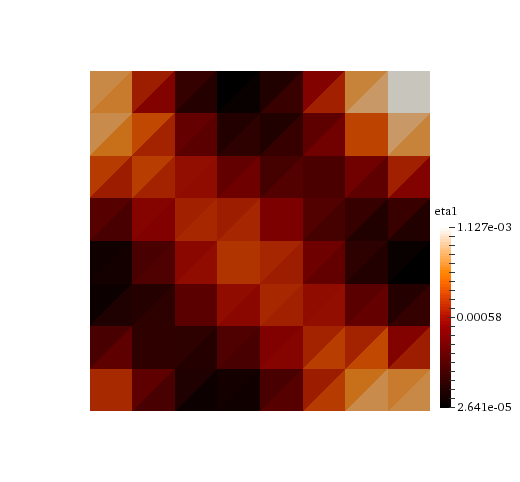
\includegraphics[width=\textwidth,height=\textheight,keepaspectratio,height=\textheight,keepaspectratio]{figures/2_mpet/no_transfer/space/eta1_8.png}
    \caption{$N=8$}
  \end{subfigure}
  \begin{subfigure}[b]{0.24\textwidth}
    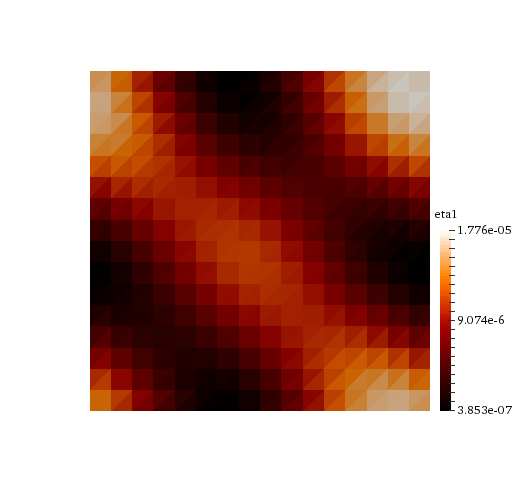
\includegraphics[width=\textwidth,height=\textheight,keepaspectratio,height=\textheight,keepaspectratio]{figures/2_mpet/no_transfer/space/eta1_16.png}
    \caption{$N=16$}
  \end{subfigure}
  \begin{subfigure}[b]{0.24\textwidth}
    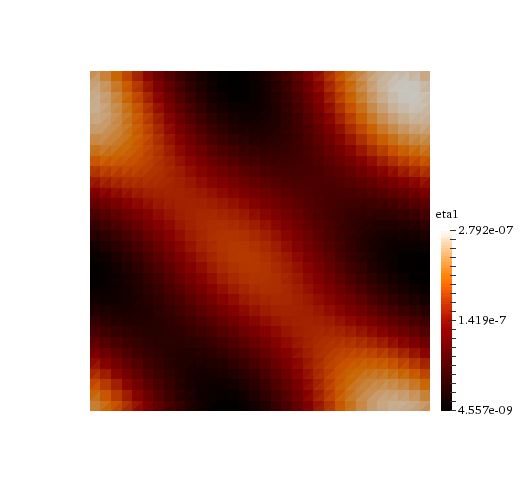
\includegraphics[width=\textwidth,height=\textheight,keepaspectratio,height=\textheight,keepaspectratio]{figures/2_mpet/no_transfer/space/eta1_32.png}
    \caption{$N=32$}
  \end{subfigure}
  \begin{subfigure}[b]{0.24\textwidth}
    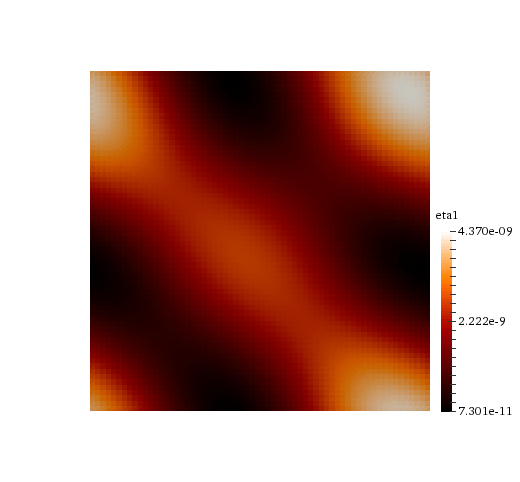
\includegraphics[width=\textwidth,height=\textheight,keepaspectratio,height=\textheight,keepaspectratio]{figures/2_mpet/no_transfer/space/eta1_64.png}
    \caption{$N=64$}
  \end{subfigure}
  \caption{Error magnitude for $\eta_1$ under space refinement at $t=T$ for two-network MPET model with interacting fluid networks} \label{fig:bb_default_eta1}
\end{figure}

\clearpage

\begin{figure}[h!]
  \centering
  \begin{subfigure}[b]{0.24\textwidth}
    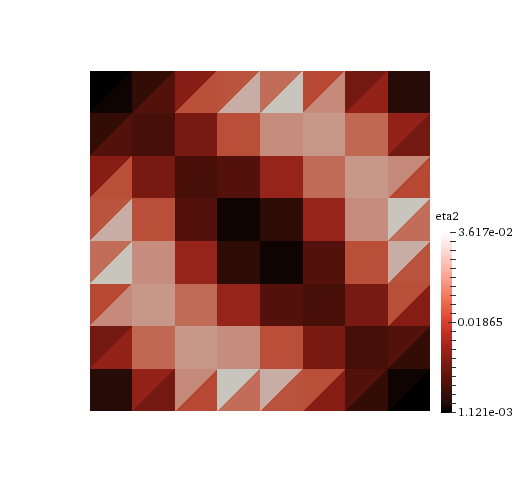
\includegraphics[width=\textwidth,height=\textheight,keepaspectratio,height=\textheight,keepaspectratio]{figures/2_mpet/no_transfer/space/eta2_8.png}
    \caption{$N=8$}
  \end{subfigure}
  \begin{subfigure}[b]{0.24\textwidth}
    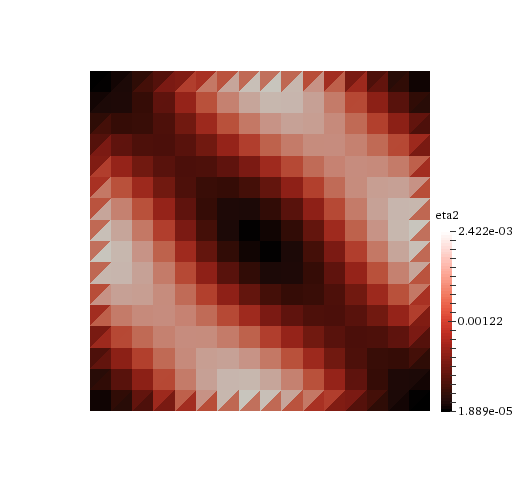
\includegraphics[width=\textwidth,height=\textheight,keepaspectratio,height=\textheight,keepaspectratio]{figures/2_mpet/no_transfer/space/eta2_16.png}
    \caption{$N=16$}
  \end{subfigure}
  \begin{subfigure}[b]{0.24\textwidth}
    \includegraphics[width=\textwidth,height=\textheight,keepaspectratio,height=\textheight,keepaspectratio]{figures/2_mpet/no_transfer/space/eta2_32.png}
    \caption{$N=32$}
  \end{subfigure}
  \begin{subfigure}[b]{0.24\textwidth}
    \includegraphics[width=\textwidth,height=\textheight,keepaspectratio,height=\textheight,keepaspectratio]{figures/2_mpet/no_transfer/space/eta2_64.png}
    \caption{$N=64$}
  \end{subfigure}
  \caption{Error magnitude for $\eta_2$ under space refinement at $t=T$ for two-network MPET model with interacting fluid networks} \label{fig:bb_default_eta2}
\end{figure}
\mbox{}\\ \\
\begin{figure}[h!]
  \centering
  \begin{subfigure}[b]{0.24\textwidth}
    \includegraphics[width=\textwidth,height=\textheight,keepaspectratio,height=\textheight,keepaspectratio]{figures/2_mpet/default/space/eta3_8.png}
    \caption{$N=8$}
  \end{subfigure}
  \begin{subfigure}[b]{0.24\textwidth}
    \includegraphics[width=\textwidth,height=\textheight,keepaspectratio,height=\textheight,keepaspectratio]{figures/2_mpet/default/space/eta3_16.png}
    \caption{$N=16$}
  \end{subfigure}
  \begin{subfigure}[b]{0.24\textwidth}
    \includegraphics[width=\textwidth,height=\textheight,keepaspectratio,height=\textheight,keepaspectratio]{figures/2_mpet/default/space/eta3_32.png}
    \caption{$N=32$}
  \end{subfigure}
  \begin{subfigure}[b]{0.24\textwidth}
    \includegraphics[width=\textwidth,height=\textheight,keepaspectratio,height=\textheight,keepaspectratio]{figures/2_mpet/default/space/eta3_64.png}
    \caption{$N=64$}
  \end{subfigure}
  \caption{Error magnitude for $\eta_3$ under space refinement at $t=T$ for two-network MPET model with interacting fluid networks} \label{fig:bb_default_eta3}
\end{figure}
\mbox{}\\ \\
\begin{figure}[h!]
  \centering
  \begin{subfigure}[b]{0.24\textwidth}
    \includegraphics[width=\textwidth,height=\textheight,keepaspectratio,height=\textheight,keepaspectratio]{figures/2_mpet/default/time/eta4_dt1.png}
    \caption{$\tau=0.01$}
  \end{subfigure}
  \begin{subfigure}[b]{0.24\textwidth}
    \includegraphics[width=\textwidth,height=\textheight,keepaspectratio,height=\textheight,keepaspectratio]{figures/2_mpet/default/time/eta4_dt2.png}
    \caption{$\tau=0.005$}
  \end{subfigure}
  \begin{subfigure}[b]{0.24\textwidth}
    \includegraphics[width=\textwidth,height=\textheight,keepaspectratio,height=\textheight,keepaspectratio]{figures/2_mpet/default/time/eta4_dt3.png}
    \caption{$\tau=0.0025$}
  \end{subfigure}
  \begin{subfigure}[b]{0.24\textwidth}
    \includegraphics[width=\textwidth,height=\textheight,keepaspectratio,height=\textheight,keepaspectratio]{figures/2_mpet/default/time/eta4_dt4.png}
    \caption{$\tau=0.00125$}
  \end{subfigure}
  \caption{Error magnitude for $\eta_4$ under time refinement at $t=T$ for two-network MPET model with interacting fluid networks} \label{fig:bb_default_eta4}
\end{figure}
\clearpage
\subsubsection{Two-network poroelasticity: physiological parameters} \label{section:num_mpet2_bio}
The main interest in using the MPET model is to simulate interacting biological fluids in a physiological setting. Thus, we perform a numerical experiment with two networks on the unit square with physiologically inspired parameters \cite{lee2018}, presented below in table \ref{tab:bb_parameters}. 
\begin{center}
\begin{tabular}{c|c|c}
Parameter & Value(s) & Unit \\\hline
$\alpha_1$  & 0.49 & -\\
$\alpha_2$  & 0.25 & -\\
$\nu$ & 0.499 & -\\
$E$ & 1500 & Pa\\
$c_1$ & $3.9 \cdot 10^{-4}$ & Pa$^{-1}$ \\
$c_2$ & $2.9 \cdot 10^{-4}$ & Pa$^{-1}$ \\
$K_1$ & $1.57 \cdot 10^{-5}$ & mm$^2$ Pa$^{-1}$ s$^{-1}$ \\
$K_2$ & $3.75 \cdot 10^{-2}$ & mm$^2$ Pa$^{-1}$ s$^{-1}$ \\
$\xi_{1}, \xi_{2}$ & 0.0 & Pa$^{-1}$ s$^{-1}$ \\
\end{tabular}
\captionof{table}{Model parameters for the two-network model for physiologically inspired numerical experiment} \label{tab:bb_parameters}
\end{center}
% gives mu = 500.033335556, lamb =  2499666.64444
Table \ref{tab:bb_bio_space_error} present the convergence rates for the a priori error estimate for the displacement and the pressures under space refinement with physiologically inspired parameters. We observe that the convergence rate for the displacement appears to increase as the mesh is refined. The pressures exhibit oscillating behavior. This is known as poroelastic locking, which occurs when the displacement is underestimated when the material is assumed to be incompressible \cite{phillips}. When some parameters are small compared to the others, the numerical approximation may become unreliable. Here, $\lambda \approx 2.499 \cdot 10^6$ and $c, K \leq 3.75 \cdot 10^{-2}$; thus the variation in the size of the parameters is considered to be large. This problem is addressed by Lee et al. \cite{lee2018}, where the proposed solution is to implement a total pressure formulation.  
\\
\\
The quantities $\eta_1$ and $\eta_3$ are approximately $10^6$ times larger compared to the first experiment with non-interacting fluid networks under space refinement. This is illustrated in table \ref{tab:bb_bio_space_est}. The estimator associated with the time error, $\eta_4$ remains constant under space refinement. Since $\eta_1$ and $\eta_3$ are dependent on the size of $\lambda$, we will expect that these quantities increase proportionally with $\lambda$. The quantities $\eta_2$ and $\eta_4$ are approximately $10^{-1}$ times smaller compared to the interactive network case with all parameters set to 2. This is expected as these estimators are dependent on the size of $c$ and $K$. In table \ref{tab:bb_bio_space_est} we observe that $\eta_1$ exhibit a slightly sub-optimal convergence, while $\eta_2$ converges optimally. The quantity $\eta_3$ converges to 1, (similarly to the single network case), that is, one order lower than optimal. The error magnitude for the space estimators $\eta_1$, $\eta_2$ and $\eta_3$ are presented in figures \ref{fig:bb_bio_eta1}, \ref{fig:bb_bio_eta2} and \ref{fig:bb_bio_eta3} respectively. We observe that the quantity detecting the residual error for the displacement under space refinement, $\eta_1$, is much larger than $\eta_3$. Recall that $\eta_3$ could heuristically be described as a measure of the change in the displacement-related spatial residual in time. As mentioned previously, this suggests a further refinement in space. 
\\
\\
Table \ref{tab:bb_bio_time_error} displays the convergence rate for the displacement and the pressures under time refinement, which indicates optimal rates for $u$ and $p_1$. The second pressure term $p_2$ exhibit tendencies of superconvergence. That is, it converges at a higher order than expected \cite{ferreira}. The error quantities $\eta_1$ and $\eta_3$ are approximately $10^6$ times larger compared to the non-interactive network experiment under time refinement, see table \ref{tab:bb_bio_time_est}. As we stated above, this is expected since they depend on the size of $\lambda$. We also observe a slightly sub-optimal convergence for $\eta_4$. $\eta_1$ and $\eta_2$ remains constant under time refinement. This is expected as they are associated with the space error. The quantity $\eta_3$ is also associated with the space error; however, it is a time-incremental version of the $\eta_1$, which results in a time-dependence. This quantity converges to 1 under time refinement. Figure  \ref{fig:bb_bio_eta4} presents the error magnitude for the time estimator $\eta_4$ under time refinement, where the lighter areas display where the error is concentrated. 
\\
\\
\begin{center} 
\centering
\begin{tabular}{c|c|c|c|c|c|c}
$h^{-1}$ & $\|u - u_{h_{\tau}}\|_{H^1}$ & Rate & $\|p_1 - p_{1h_{\tau}}\|_{L^2}$ & Rate & $\|p_2 - p_{2h_{\tau}}\|_{L^2}$ & Rate\\\hline
4  & 8.125e-2 & -     & 5.458e-1 & -     & 5.131e-3 & -     \\
8  & 4.449e-2 & 0.869 & 2.537e-2 & 4.427 & 1.652e-3 & 1.635 \\
16 & 1.854e-2 & 1.263 & 1.303e-2 & 0.962 & 4.495e-4 & 1.878 \\
32 & 5.563e-3 & 1.737 & 1.468e-2 & -0.172 & 1.383e-4 & 1.700 \\
64 & 1.203e-3 & 2.209 & 1.476e-2 & -0.008 & 8.532e-5 & 0.697 \\\hline
Opt. & & 2 & & 2 & & 2
\end{tabular}
\captionof{table}{Error norms and convergence rates for two network MPET model under space refinement, $T=0.1$, $\tau = 5.0$e-5, with physiologically inspired parameters} \label{tab:bb_bio_space_error}
\end{center}
\mbox{}\\ \\ \\
\begin{center} 
\centering
\begin{tabular}{c|c|c|c|c|c|c|c}
$h^{-1}$ & $\eta_1$ & Rate &  $\eta_2$ & Rate & $\eta_3$ & Rate & $\eta_4$ \\\hline
4  & 1.123e+6 & -     & 1.302e-2 & -     & 1.905e+3 & -     & 3.874e-5 \\
8  & 2.830e+5 & 1.989 & 7.381e-3 & 0.819 & 9.651e+2 & 0.981 & 3.966e-5 \\
16 & 7.143e+4 & 1.986 & 3.855e-3 & 0.937 & 4.841e+2 & 0.996 & 3.995e-5 \\
32 & 1.816e+4 & 1.975 & 1.958e-3 & 0.997 & 2.422e+2 & 0.999 & 4.003e-5 \\
64 & 4.634e+3 & 1.971 & 9.854e-4 & 0.991 & 1.211e+2 & 1.000 & 4.005e-5 \\\hline
Opt. & & 2 & & 1  & & 2 & 
\end{tabular}
\captionof{table}{Convergence rate for a posteriori error estimates for two network MPET model under space refinement, $T=0.1$, $\tau = 5.0$e-5, with physiologically inspired parameters} \label{tab:bb_bio_space_est}
\end{center}

\clearpage

\begin{center} 
\centering
\small
\begin{tabular}{c|c|c|c|c|c|c}
$\tau$ & $\|u-u_{h_{\tau}}\|_{H^1}$ & Rate & $\|p_1-p_{1h_{\tau}}\|_{L^2}$ & Rate & $\|p_2-p_{2h_{\tau}}\|_{L^2}$ & Rate \\\hline
0.02   	& 4.602e-5 & -     & 1.704e+2 & -     & 8.891e-3 &  -    \\
0.01   	& 2.300e-5 & 1.001 & 8.492e+1 & 1.005 & 2.258e-3 & 1.977 \\
0.005  	& 1.149e-5 & 1.001 & 4.238e+1 & 1.003 & 5.811e-4 & 1.958 \\
0.0025  & 5.746e-6 & 1.000 & 2.117e+1 & 1.001 & 1.535e-4 & 1.920 \\
0.00125 & 2.873e-6 & 1.000 & 1.058e+1 & 1.001 & 4.251e-5 & 1.853 \\ \hline
Opt. & & 1 & & 1  & & 1
\end{tabular}
\normalsize
\captionof{table}{Error estimates and convergence rates for the two network MPET model with interacting fluid networks under time refinement, $T=1$, $h=1/64$, with physiologically inspired parameters} \label{tab:bb_bio_time_error}
\end{center}
\mbox{} \\ \\ \\ 
\begin{center} 
\centering
\begin{tabular}{c|c|c|c|c|c}
$\tau$ & $\eta_1$ & $\eta_2$ & $\eta_3$ & $\eta_4$ & Rate\\\hline
0.02    & 3.801e+3 & 3.268e-3 & 2.421e+4 & 8.249e-2 & -    \\
0.01    & 3.801e+3 & 3.194e-3 & 1.211e+4 & 2.643e-2 & 1.642\\
0.005   & 3.801e+3 & 3.175e-3 & 6.057e+3 & 1.057e-2 & 1.322\\
0.0025  & 3.801e+3 & 3.171e-3 & 3.029e+3 & 4.905e-3 & 1.108\\
0.00125 & 3.801e+3 & 3.169e-3 & 1.514e+3 & 2.404e-3 & 1.029\\\hline
Opt. & & & & & 1
\end{tabular}
\captionof{table}{A posteriori error and convergence rates for the two network MPET model with interacting fluid networks under time refinement, $T=1$, $h=1/64$, with physiologically inspired parameters} \label{tab:bb_bio_time_est}
\end{center}
\mbox{}\\ \\ \\ \\
\begin{figure}[h!]
  \centering
  \begin{subfigure}[b]{0.24\textwidth}
    \includegraphics[width=\textwidth,height=\textheight,keepaspectratio,height=\textheight,keepaspectratio]{figures/2_mpet/biomedical/space/eta1_8.png}
    \caption{$N=8$}
  \end{subfigure}
  \begin{subfigure}[b]{0.24\textwidth}
    \includegraphics[width=\textwidth,height=\textheight,keepaspectratio,height=\textheight,keepaspectratio]{figures/2_mpet/biomedical/space/eta1_16.png}
    \caption{$N=16$}
  \end{subfigure}
  \begin{subfigure}[b]{0.24\textwidth}
    \includegraphics[width=\textwidth,height=\textheight,keepaspectratio,height=\textheight,keepaspectratio]{figures/2_mpet/biomedical/space/eta1_32.png}
    \caption{$N=32$}
  \end{subfigure}
  \begin{subfigure}[b]{0.24\textwidth}
    \includegraphics[width=\textwidth,height=\textheight,keepaspectratio,height=\textheight,keepaspectratio]{figures/2_mpet/biomedical/space/eta1_64.png}
    \caption{$N=64$}
  \end{subfigure}
  \caption{Error magnitude for $\eta_1$ under space refinement at $t=T$ for two-network MPET model with physiologically inspired parameters} \label{fig:bb_bio_eta1}
\end{figure}

\clearpage

\begin{figure}[h!]
  \centering
  \begin{subfigure}[b]{0.24\textwidth}
    \includegraphics[width=\textwidth,height=\textheight,keepaspectratio,height=\textheight,keepaspectratio]{figures/2_mpet/biomedical/space/eta2_8.png}
    \caption{$N=8$}
  \end{subfigure}
  \begin{subfigure}[b]{0.24\textwidth}
    \includegraphics[width=\textwidth,height=\textheight,keepaspectratio,height=\textheight,keepaspectratio]{figures/2_mpet/biomedical/space/eta2_16.png}
    \caption{$N=16$}
  \end{subfigure}
  \begin{subfigure}[b]{0.24\textwidth}
    \includegraphics[width=\textwidth,height=\textheight,keepaspectratio,height=\textheight,keepaspectratio]{figures/2_mpet/biomedical/space/eta2_32.png}
    \caption{$N=32$}
  \end{subfigure}
  \begin{subfigure}[b]{0.24\textwidth}
    \includegraphics[width=\textwidth,height=\textheight,keepaspectratio,height=\textheight,keepaspectratio]{figures/2_mpet/biomedical/space/eta2_64.png}
    \caption{$N=64$}
  \end{subfigure}
  \caption{Error magnitude for $\eta_2$ under space refinement at $t=T$ for two-network MPET model with physiologically inspired parameters} \label{fig:bb_bio_eta2}
\end{figure}
\mbox{}\\ \\
\begin{figure}[h!]
  \centering
  \begin{subfigure}[b]{0.24\textwidth}
    \includegraphics[width=\textwidth,height=\textheight,keepaspectratio,height=\textheight,keepaspectratio]{figures/2_mpet/biomedical/space/eta3_8.png}
    \caption{$N=8$}
  \end{subfigure}
  \begin{subfigure}[b]{0.24\textwidth}
    \includegraphics[width=\textwidth,height=\textheight,keepaspectratio,height=\textheight,keepaspectratio]{figures/2_mpet/biomedical/space/eta3_16.png}
    \caption{$N=16$}
  \end{subfigure}
  \begin{subfigure}[b]{0.24\textwidth}
    \includegraphics[width=\textwidth,height=\textheight,keepaspectratio,height=\textheight,keepaspectratio]{figures/2_mpet/biomedical/space/eta3_32.png}
    \caption{$N=32$}
  \end{subfigure}
  \begin{subfigure}[b]{0.24\textwidth}
    \includegraphics[width=\textwidth,height=\textheight,keepaspectratio,height=\textheight,keepaspectratio]{figures/2_mpet/biomedical/space/eta3_64.png}
    \caption{$N=64$}
  \end{subfigure}
  \caption{Error magnitude for $\eta_3$ under space refinement at $t=T$ for two-network MPET model with physiologically inspired parameters} \label{fig:bb_bio_eta3}
\end{figure}
\mbox{}\\ \\
\begin{figure}[h!]
  \centering
  \begin{subfigure}[b]{0.24\textwidth}
    \includegraphics[width=\textwidth,height=\textheight,keepaspectratio,height=\textheight,keepaspectratio]{figures/2_mpet/biomedical/time/eta4_dt1.png}
    \caption{$\tau=0.01$}
  \end{subfigure}
  \begin{subfigure}[b]{0.24\textwidth}
    \includegraphics[width=\textwidth,height=\textheight,keepaspectratio,height=\textheight,keepaspectratio]{figures/2_mpet/biomedical/time/eta4_dt2.png}
    \caption{$\tau=0.005$}
  \end{subfigure}
  \begin{subfigure}[b]{0.24\textwidth}
    \includegraphics[width=\textwidth,height=\textheight,keepaspectratio,height=\textheight,keepaspectratio]{figures/2_mpet/biomedical/time/eta4_dt3.png}
    \caption{$\tau=0.0025$}
  \end{subfigure}
  \begin{subfigure}[b]{0.24\textwidth}
    \includegraphics[width=\textwidth,height=\textheight,keepaspectratio,height=\textheight,keepaspectratio]{figures/2_mpet/biomedical/time/eta4_dt4.png}
    \caption{$\tau=0.00125$}
  \end{subfigure}
  \caption{Error magnitude for $\eta_4$ under time refinement at $t=T$ for two-network model with physiologically inspired parameters} \label{fig:bb_bio_eta4}
\end{figure}
\clearpage

\subsection{Four-network poroelasticity} \label{test_mpet4}
As stated in the introduction, the primary motivation in using the MPET equations is to use them to model fluid transportation in the brain. In light of this, it is essential to be able to control the error on complex geometries. Thus, we present the a posteriori error magnitudes for a four-network MPET model on a mouse brain mesh, see figure \ref{fig:brain_mesh}. These experiments as purely meant as a demonstration of how the a posteriori error estimators will work on a geometry different from the unit square. In addition, the experiment implements the a posteriori error estimates derived for the two network poroelasticity model in chapter \ref{chap:error}, however, extended to four networks which demonstrates that the analytic results do not depend on the network number. 
\\
\\ 
For the four-network poroelasticity model we use the following manufactured solution,
\begin{align*}
u_e = & \, \left(\cos(\pi x)\sin(\pi y)\sin(\pi t), \, \sin( \pi x)\cos(\pi y)\sin(\pi t)\right) \\
p_{1_e} = & = p_{2_e} = p_{3_e} = p_{4_e} \,\sin(\pi x) \sin(\pi y)\sin(2\pi t)  
\end{align*}
We consider the entire boundary to be under clamped conditions with Dirichlet data given by the method of manufactured solution for simplicity. It is important to point out that these boundary conditions are not biophysical, but merely prescribed as a demonstration. Clamped boundary conditions are considered much more accessible to implement than the more comprehensive boundary conditions presented in, e.g. \cite{vardakis}. 
\\
\begin{figure}[h!]
\centering
  \includegraphics[scale=0.5]{figures/4_mpet/biomedical/brain_mesh.png}
  \caption[Caption for LOF]{Mouse brain mesh\footnotemark{} with 39409 cells }
  \label{fig:brain_mesh}
\end{figure}
\footnotetext{   \textcopyright Janis Grobovs, Alexandra Diem and the Allen Mouse Brain Atlas}
\mbox{}\\
The estimator associated with the displacement-related spatial residual under uniform space refinement is displayed in figure \ref{fig:mpet4_eta1}. Only one uniform spatial refinement was performed, as this is a computationally expensive procedure. The estimator describing the pressure-related spatial residual are presented in figures \ref{fig:mpet4_eta2_p1}, \ref{fig:mpet4_eta2_p2}, \ref{fig:mpet4_eta2_p3} and \ref{fig:mpet4_eta2_p4} for the four pressure components, respectively. The first pressure term $p_1$ behaves differently compared to the three other components. That is $p_2$, $p_3$ and $p_4$ exhibit larger concentration of error compared to $p_1$. This suggests that an adaptive refinement process should target $p_2$, $p_3$ and $p_4$. Figure \ref{fig:mpet4_eta3} displays the estimator that measures the change in the displacement-related spatial residual in time. We observe that this estimator yields minimal errors, which suggests that a smaller time step is not necessary to ensure a better refinement in space. The time estimator for each pressure component under time refinement is presented in figure \ref{fig:mpet4_eta4}. Each pressure component exhibits similar error concentrations under time refinement, where we observe that the error decreases as the time step decreases. One important feature of the error estimates is to be able to identify the areas where the error is high; this becomes clearer as we refine uniformly. That is, the resolution increases and we are consequently able to locate the specific areas in need of refinement. This experiment demonstrates how the error is distributed on a complex geometry for each error component. 
\begin{figure}[h!]
  \centering
  \begin{subfigure}[b]{0.49\textwidth}
    \includegraphics[width=\textwidth,height=\textheight,keepaspectratio,height=\textheight,keepaspectratio]{figures/4_mpet/biomedical/space/eta1_1.png}
    \caption{39409 mesh cells}
  \end{subfigure}
  \begin{subfigure}[b]{0.49\textwidth}
    \includegraphics[width=\textwidth,height=\textheight,keepaspectratio,height=\textheight,keepaspectratio]{figures/4_mpet/biomedical/space/eta1_2.png}
    \caption{157636 mesh cells}
  \end{subfigure}
  \caption{Error magnitude for $\eta_1$ under uniform space refinement at $t=T$ for four-network MPET model with physiologically inspired parameters on brain mesh} \label{fig:mpet4_eta1}
\end{figure}


\begin{figure}[h!]
  \centering
  \begin{subfigure}[b]{0.49\textwidth}
    \includegraphics[width=\textwidth,height=\textheight,keepaspectratio,height=\textheight,keepaspectratio]{figures/4_mpet/biomedical/space/eta2_p1_1.png}
    \caption{39409 mesh cells}
  \end{subfigure}
  \begin{subfigure}[b]{0.49\textwidth}
    \includegraphics[width=\textwidth,height=\textheight,keepaspectratio,height=\textheight,keepaspectratio]{figures/4_mpet/biomedical/space/eta2_p1_2.png}
    \caption{157636 mesh cells}
  \end{subfigure}
  \caption{Error magnitude for $\eta_2$ associated with the pressure $p_1$ under uniform space refinement at $t=T$ for four-network MPET model with physiologically inspired parameters on brain mesh} \label{fig:mpet4_eta2_p1}
\end{figure}

\begin{figure}[h!]
  \centering
    \begin{subfigure}[b]{0.49\textwidth}
    \includegraphics[width=\textwidth,height=\textheight,keepaspectratio,height=\textheight,keepaspectratio]{figures/4_mpet/biomedical/space/eta2_p2_1.png}
    \caption{39409 mesh cells}
  \end{subfigure}
  \begin{subfigure}[b]{0.49\textwidth}
    \includegraphics[width=\textwidth,height=\textheight,keepaspectratio,height=\textheight,keepaspectratio]{figures/4_mpet/biomedical/space/eta2_p2_2.png}
    \caption{157636 mesh cells}
  \end{subfigure}
  \caption{Error magnitude for $\eta_2$ associated with the pressure $p_2$ under uniform space refinement at $t=T$ for four-network MPET model with physiologically inspired parameters on brain mesh} \label{fig:mpet4_eta2_p2}
\end{figure}

\begin{figure}[h!]
  \centering
    \begin{subfigure}[b]{0.49\textwidth}
    \includegraphics[width=\textwidth,height=\textheight,keepaspectratio,height=\textheight,keepaspectratio]{figures/4_mpet/biomedical/space/eta2_p3_1.png}
    \caption{39409 mesh cells}
  \end{subfigure}
  \begin{subfigure}[b]{0.49\textwidth}
    \includegraphics[width=\textwidth,height=\textheight,keepaspectratio,height=\textheight,keepaspectratio]{figures/4_mpet/biomedical/space/eta2_p3_2.png}
    \caption{157636 mesh cells}
  \end{subfigure}
  \caption{Error magnitude for $\eta_2$ associated with the pressure $p_3$ under uniform space refinement at $t=T$ for four-network MPET model with physiologically inspired parameters on brain mesh} \label{fig:mpet4_eta2_p3}
\end{figure}

\begin{figure}[h!]
  \centering
    \begin{subfigure}[b]{0.49\textwidth}
    \includegraphics[width=\textwidth,height=\textheight,keepaspectratio,height=\textheight,keepaspectratio]{figures/4_mpet/biomedical/space/eta2_p4_1.png}
    \caption{39409 mesh cells}
  \end{subfigure}
  \begin{subfigure}[b]{0.49\textwidth}
    \includegraphics[width=\textwidth,height=\textheight,keepaspectratio,height=\textheight,keepaspectratio]{figures/4_mpet/biomedical/space/eta2_p4_2.png}
    \caption{157636 mesh cells}
  \end{subfigure}
  \caption{Error magnitude for $\eta_2$ associated with the pressure $p_4$ under uniform space refinement at $t=T$ for four-network MPET model with physiologically inspired parameters on brain mesh} \label{fig:mpet4_eta2_p4}
\end{figure}


\begin{figure}[h!]
  \centering
  \centering
    \begin{subfigure}[b]{0.49\textwidth}
    \includegraphics[width=\textwidth,height=\textheight,keepaspectratio,height=\textheight,keepaspectratio]{figures/4_mpet/biomedical/space/eta3_1.png}
    \caption{39409 mesh cells}
  \end{subfigure}
  \begin{subfigure}[b]{0.49\textwidth}
    \includegraphics[width=\textwidth,height=\textheight,keepaspectratio,height=\textheight,keepaspectratio]{figures/4_mpet/biomedical/space/eta3_2.png}
    \caption{157636 mesh cells}
  \end{subfigure}
  \caption{Error magnitude for $\eta_3$ under uniform space refinement at $t=T$ for four-network MPET model with physiologically inspired parameters on a brain mesh} \label{fig:mpet4_eta3}
\end{figure}

\begin{figure}[h!]
  \centering
  \begin{subfigure}[b]{0.24\textwidth}
    \includegraphics[width=\textwidth,height=\textheight,keepaspectratio,height=\textheight,keepaspectratio]{figures/4_mpet/biomedical/time/eta4_p1_dt1.png}
    \caption{$p_1$, $\tau=0.01$}
  \end{subfigure}
  \begin{subfigure}[b]{0.24\textwidth}
    \includegraphics[width=\textwidth,height=\textheight,keepaspectratio,height=\textheight,keepaspectratio]{figures/4_mpet/biomedical/time/eta4_p1_dt2.png}
    \caption{$p_1$, $\tau=0.005$}
  \end{subfigure}
  \begin{subfigure}[b]{0.24\textwidth}
    \includegraphics[width=\textwidth,height=\textheight,keepaspectratio,height=\textheight,keepaspectratio]{figures/4_mpet/biomedical/time/eta4_p1_dt3.png}
    \caption{$p_1$, $\tau=0.0025$}
  \end{subfigure}
  \begin{subfigure}[b]{0.24\textwidth}
    \includegraphics[width=\textwidth,height=\textheight,keepaspectratio,height=\textheight,keepaspectratio]{figures/4_mpet/biomedical/time/eta4_p1_dt4.png}
    \caption{$p_1$, $\tau=0.00125$}
  \end{subfigure}
  \begin{subfigure}[b]{0.24\textwidth}
    \includegraphics[width=\textwidth,height=\textheight,keepaspectratio,height=\textheight,keepaspectratio]{figures/4_mpet/biomedical/time/eta4_p2_dt1.png}
    \caption{$p_2$, $\tau=0.01$}
  \end{subfigure}
  \begin{subfigure}[b]{0.24\textwidth}
    \includegraphics[width=\textwidth,height=\textheight,keepaspectratio,height=\textheight,keepaspectratio]{figures/4_mpet/biomedical/time/eta4_p2_dt2.png}
    \caption{$p_2$, $\tau=0.005$}
  \end{subfigure}
  \begin{subfigure}[b]{0.2\textwidth}
    \includegraphics[width=\textwidth,height=\textheight,keepaspectratio,height=\textheight,keepaspectratio]{figures/4_mpet/biomedical/time/eta4_p2_dt3.png}
    \caption{$p_2$, $\tau=0.0025$}
  \end{subfigure}
  \begin{subfigure}[b]{0.24\textwidth}
    \includegraphics[width=\textwidth,height=\textheight,keepaspectratio,height=\textheight,keepaspectratio]{figures/4_mpet/biomedical/time/eta4_p2_dt4.png}
    \caption{$p_2$, $\tau=0.00125$}
  \end{subfigure}
  \begin{subfigure}[b]{0.24\textwidth}
    \includegraphics[width=\textwidth,height=\textheight,keepaspectratio,height=\textheight,keepaspectratio]{figures/4_mpet/biomedical/time/eta4_p3_dt1.png}
    \caption{$p_3$, $\tau=0.01$}
  \end{subfigure}
  \begin{subfigure}[b]{0.24\textwidth}
    \includegraphics[width=\textwidth,height=\textheight,keepaspectratio,height=\textheight,keepaspectratio]{figures/4_mpet/biomedical/time/eta4_p3_dt2.png}
    \caption{$p_3$, $\tau=0.005$}
  \end{subfigure}
  \begin{subfigure}[b]{0.24\textwidth}
    \includegraphics[width=\textwidth,height=\textheight,keepaspectratio,height=\textheight,keepaspectratio]{figures/4_mpet/biomedical/time/eta4_p3_dt3.png}
    \caption{$p_3$, $\tau=0.0025$}
  \end{subfigure}
  \begin{subfigure}[b]{0.24\textwidth}
    \includegraphics[width=\textwidth,height=\textheight,keepaspectratio,height=\textheight,keepaspectratio]{figures/4_mpet/biomedical/time/eta4_p3_dt4.png}
    \caption{$p_3$, $\tau=0.00125$}
  \end{subfigure}

  \begin{subfigure}[b]{0.24\textwidth}
    \includegraphics[width=\textwidth,height=\textheight,keepaspectratio,height=\textheight,keepaspectratio]{figures/4_mpet/biomedical/time/eta4_p4_dt1.png}
    \caption{$p_4$, $\tau=0.01$}
  \end{subfigure}
  \begin{subfigure}[b]{0.24\textwidth}
    \includegraphics[width=\textwidth,height=\textheight,keepaspectratio,height=\textheight,keepaspectratio]{figures/4_mpet/biomedical/time/eta4_p4_dt2.png}
    \caption{$p_4$, $\tau=0.005$}
  \end{subfigure}
  \begin{subfigure}[b]{0.24\textwidth}
    \includegraphics[width=\textwidth,height=\textheight,keepaspectratio,height=\textheight,keepaspectratio]{figures/4_mpet/biomedical/time/eta4_p4_dt3.png}
    \caption{$p_4$, $\tau=0.0025$}
  \end{subfigure}
  \begin{subfigure}[b]{0.24\textwidth}
    \includegraphics[width=\textwidth,height=\textheight,keepaspectratio,height=\textheight,keepaspectratio]{figures/4_mpet/biomedical/time/eta4_p4_dt4.png}
    \caption{$p_4$, $\tau=0.00125$}
  \end{subfigure}
  \begin{subfigure}[b]{0.5\textwidth}
    \includegraphics[width=\textwidth,height=\textheight,keepaspectratio,height=\textheight,keepaspectratio]{figures/4_mpet/biomedical/time/eta4_range.png}
  \end{subfigure}
  \caption{Error magnitude for $\eta_4$ associated with pressure terms $p_1$, $p_2$, $p_3$ and $p_4$ (in order) under time refinement at $t=T$ for four-network model with physiologically inspired parameters} \label{fig:mpet4_eta4}
\end{figure}
